\documentclass[10pt]{report}
\usepackage{fancyhdr, amsmath, amsthm, amssymb, enumerate, tikz, hyperref}
\usepackage[margin=0.5in, top=0.8in, bottom=0.8in]{geometry}
\usepackage[version=3]{mhchem}
\newcommand{\scinot}[2]{#1\times 10^{#2}}
\newcommand{\rtd}[2]{\frac{d^2#1}{d#2^2}}
\newcommand{\ptd}[2]{\frac{\partial^2 #1}{\partial#2^2}}
\newcommand{\bra}[1]{\left<#1\right|}
\newcommand{\ket}[1]{\left|#1\right>}
\newcommand{\dotp}[2]{\left<#1\left.\right|#2\right>}
\newcommand{\rd}[2]{\frac{d#1}{d#2}}
\newcommand{\pd}[2]{\frac{\partial #1}{\partial#2}}
\newcommand{\norm}[1]{\left|\left|#1\right|\right|}
\newcommand{\abs}[1]{\left|#1\right|}
\newcommand{\Log}[0]{\mathrm{Log} }
\newcommand{\Arg}[0]{\mathrm{Arg} }
\newcommand{\Res}[0]{\mathrm{Res} }
\DeclareMathOperator{\erfc}{erfc}
\newcommand{\tr}[0]{\mathrm{tr} }
\usepackage[labelfont=bf, font=scriptsize]{caption}
\everymath{\displaystyle}

\begin{document}

\pagestyle{fancy}
\rhead{Yubo Su --- ACM95c --- Greg Rizza}
\title{ACM95 --- KRK 119 --- MWF 11-12}
\author{Yubo Su}
\date{ }

\maketitle

\tableofcontents
\newpage

\chapter{Key Concepts}

\begin{itemize}
    \item Transformation matrix (basis change) is given $A_{ik} = \hat{f}_i\cdot \hat{e}_k$ and takes $A_{ik}v_k^e = v_i^f$ for some bases $\left\{ \hat{e}_i  \right\}, \left\{ \hat{f}_i  \right\}$. Vectors/tensors transform as
        $$\vec{v}^{\,f} = \mathbf{A}\vec{v}^{\,e}\;\;\;\;\;\;\;\;\;\;\;\; \mathbf{S}^f = \mathbf{A}\mathbf{S}^e\mathbf{A}^T$$
    \item Orthogonal tensor defined $\mathbf{Q}^{-1} = \mathbf{Q}^T$ and $\det(\mathbf{Q}) = \pm 1$. Positive determinant is proper orthogonal tensor, rigid rotation, and negative is improper, reflection. 
    \item Tensor product $\vec{a} \otimes \vec{b}$ is defined such that $(\vec{a}\otimes \vec{b})\vec{v} = (\vec{b}\cdot \vec{v})\vec{a}$.
    \item Only symmetric matricies can be positive definite.
    \item Heat conduction equation $\pd{u}{t} = -\pd{\phi}{x_1} + Q$ can reduce into $\pd{u}{t} = K \ptd{u}{x}$ for $Q = 0$, $K = \frac{k_0}{c\rho}$. If we then assume a bunch more stuff we can turn this into form $\nabla^2 u = 0$.
    \item Solving Laplace's equation has two ansatz's, separation of variables $u(x_i,t) = X_i(x_i)T(t)$ and \emph{similarity solution}. This fiats that for some variable $\eta_i = \frac{x_i}{\sqrt{kt}}$ that $u(x_i,t) = t^pg(\eta_i)$ with $p$ constant.
    \item Solving functions by Laplace/Fourier transform is pretty important; see lectures 5/5-5/7. Convolution theores are key to doing this.
    \item Separation of variables oftentimes ends up being eigenfunction expansion, see 5/9.
    \item For inhomogeneous BCs use \emph{method of finite transforms}: use a change of variables $\phi(x,t) = \psi(x,t) + g(t) I_0(x) + h(t)I_L(x)$ with $I_0(0) = 1, I_0(L) = 0, I_L(0) = 0, I_L(L) = 1$, because now $\psi(x,t)$ satisfies good BCs.
    \item Heat equation $\pd{U}{t} = \nabla^2 U$ vs. wave equation $\ptd{U}{t} = \nabla^2 U$ vs. Helmholtz equation $\nabla^2 \phi + \lambda \phi =0$ are the big PDEs. 
\end{itemize}

\chapter{3/31/14-4/4/14 --- Introduction, Notation Stuff} 

We will be using Moodle. Enrollment key is ``laplace.'' We will review the syllabus, so zzzz time. Topics are
\begin{itemize}
    \item Review of BVP
    \item Tensor analysis/coordinate systems
    \item Intro to linear PDEs
    \item Heat equation, Poisson/Laplace equation
    \item Wave equation
    \item Green's Functions
    \item Intro to Navier-Stokes Equation and applications (if time permits)
\end{itemize}

Note that there will be two midterms and a cumulative final, all will be split up into in class/take home portions. Only hand written notes will be allowed on in class portions. There will be only four homeworks for the entire term!! Posted on Monday, due on monday 10AM at Steele. HW is 15\%, Midterms will be 15\% on the weaker and 30\% on the stronger portions, and final is 40\%.


We begin with tensor/vector analysis. We define $\abs{\vec{v}} = v$ the magnitude of the vector, and we will define the \emph{components} of a vector to be its components along an orthonormal basis, the $\left\{ \hat{e}_i \right\}$ unit vectors. They are mutually orthogonal and form a right-handed triad. The copmonents of a vector are then $\vec{v} = v_1\hat{e}_1 + v_2\hat{e}_2 + v_3\hat{e}_3$ with the $v_i$ the components in the $\left\{ \hat{e}_i \right\}$ basis.

We will adopt the \emph{Einstein Notation} where $\vec{v} = v_i\hat{e}_i$, omitting the summation symbol, e.g. $\vec{v}\cdot \hat{e}_j$ is three separate equations.

We will also introduce the Kronecker delta notation $\hat{e}_i \cdot \hat{e}_j = \delta_{ij}$ when $\hat{e}_i$ are orthonormal, i.e. $\vec{v}\cdot \hat{e}_j = \vec{v}_i\delta_{ij}$.

We can use our newfound powers to practice writing dotting vectors. 
\begin{align}
    \vec{a}\cdot \vec{b} &= \vec{a}\cdot b_i\hat{e}_i\\
    &= a_i\hat{e}_i\cdot b_j\hat{e}_j\\
    &= a_ib_i
\end{align}

Woohoo! We're so powerful now. We eventually want to be able to transform basis vectors. 


Note that dot products are \emph{projections} of one vector on another, i.e. finding component along unit basis vector. Dotting with some non-unit vector is a projection onto the vector but multiplied by the magnitude of the other target vector, i.e. $\vec{a} \cdot\vec{b} = \abs{a}\abs{b}\cos\theta$.

Free indicies repeat independently, such as $(a\cdot b)(c \cdot d)\vec{c} = \vec{d}$ is also written $a_kb_kc_ib_ic_j = d_j$.

We've already talked about the Kronecker Delta, but something else useful is the \emph{permutation/alternating symbol} (Levi-Civita operator?\dots), as below
\begin{equation}
    \epsilon_{ijk} = 
    \begin{cases}
        1& \mbox{if } \text{cyclic}\\
        -1& \mbox{if } \text{acyclic}\\
        0& \mbox{else}
    \end{cases}
\end{equation}

Cross products are then
\begin{align}
    \vec{c} &= \vec{a} \times \vec{b}& c_i &= \epsilon_{ijk}a_j b_k
\end{align}

Then $\vec{b}\times \vec{a} = -\vec{a}\times\vec{b}$. Moreover we can examine $\vec{c}\cdot \vec{a} = \epsilon_{ijk}a_jb_ka_i = -\epsilon_{jik}a_jb_ka_i$ which then clearly must vanish, so $(a \times b) \cdot a = 0$ thankfully.

Permutation identities. First
\begin{align}
    \epsilon_{ijk}\epsilon_{ipq} &= \delta_{jp}\delta_{kq} - \delta_{jq}\delta_{kp}
\end{align}

We can see this by rewriting $\vec{c} = \vec{a} \times \vec{b}$ as $c_i^2 = \epsilon_{ijk}a_jb_k \epsilon_{ipq}a_pb_q$ and then noting that $\abs{c}^2 = c_i^2 = \abs{a}^2 \abs{b}^2 - (a\cdot b)^2$ (identity we will prove in HW, sweet) we obtain
\begin{align}
    c_i^2 &= a_n^2b_m^2 - a_rb_r a_sb_s\\
    &= a_j\delta_{nj}a_p\delta_{np}b_k\delta_{mk}b_q\delta_{mq} - a_j\delta_{rj}b_q\delta_{qr} a_s\delta_{sp}b_k\delta_{sk}\\
    &= a_ja_p\delta_{jp}b_kb_q\delta_{kq} - a_jb_q\delta_{qj} a_pb_k\delta_{pk}\\
    \abs{a \times b}^2 &= \epsilon_{ijk}a_jb_k \epsilon_{ipq}a_pb_q
\end{align}

Then factoring out $a_jb_ka_pb_q$ we obtain our answer.

Quick blurb on where vector products occur, principal invariants! Determinant of a matrix $I_3 = \det(S) = \frac{1}{6}\epsilon_{ijk}\epsilon_{pqr}S_{ip}S_{jq}S_{kr}$ is invariant, true for all tensors.

Another place where vector products pop up is in torques, where $\vec{\tau} = \vec{d}\times \vec{F}$.

\chapter{4/7/14 --- Change of basis}

How do we change basis for vectors? Exhibit two bases $\left\{ \hat{e} _i \right\}, \left\{ \hat{f} _i \right\}$ with $i \in [1,3]$ of course. Introduce $\vec{v}$ with components $v_i^{e,f}$ in the respective bases, i.e. $v_i^e = \vec{v}\cdot \hat{e}_i$. Then
\begin{align}
    v_i^f &= \vec{v}\cdot\hat{f}_i = v_k^e\hat{e}_k\cdot \hat{f}_i = \left( \hat{f}_i\cdot \hat{e}_k   \right)v_k^e   
\end{align}

Thus $\hat{f}_i\cdot \hat{e}_k = A_{ik}$ the \emph{Transformation Matrix} which we multiply $v_k^e$ to $v_i^f$. Similarly $A_{ki} = \hat{f}_k\cdot \hat{e}_i$ takes $v_k^f \to v_i^e$; note that it is just the transpose of the other transformation matrix. Note that $\mathbf{A}$ must then be orthogonal, $\mathbf{A}\mathbf{A}^T = I$. We can see this in index form
\begin{align}
    v_k^f &= A_{ki}A_{ij}v_j^f = \delta_{kj}v_j^f
\end{align}
where we get the Kronecker delta because $v_k^f = \delta_{kj}v_j^f$; we equate two representations above.

We then want to look at basis-independent functions, e.g. dot product
\begin{align}
    \vec{a}\cdot\vec{b} &= a_i^e b_i^e\\
    &= A_ika_k^fA_{ip}b_p^f\\
    &= \delta_{kp}a_k^fb_p^f\\
    &= a_k^fb_k^f
\end{align}

Let's then try to go from cartesian to polar (cylindrical, not spherical) coordinates, $\left\{ \hat{e}_1, \hat{e}_2, \hat{e}_3 \right\}\to \left\{ \hat{e}_r, \hat{e}_\theta, \hat{e}_z \right\}$. Exhibit vector $\vec{v}$. We then note that $v_3 = v_z$ by construction, so we have to find the transformation rules for the other two components. A quick geometric argument shows (messy notation; $\Rightarrow$ denotes ``contributes to'')
\begin{align}
    v_r\hat{e}_r\cos\theta &\Rightarrow v_1\hat{e}_1 & v_r\hat{e}_r\sin\theta &\Rightarrow v_2\hat{e}_2\\
    v_\theta\hat{e}_\theta(-\sin\theta) &\Rightarrow v_1\hat{e}_1 & v_\theta \hat{e}_\theta\cos\theta &\Rightarrow v_2\hat{e}_2
\end{align}
\begin{align}
    \begin{pmatrix} v_1\\v_2\\v_3 \end{pmatrix} &= \underbrace{\begin{bmatrix} \cos\theta  & -\sin\theta & 0\\\sin\theta & \cos\theta & 0\\0 & 0 & 1 \end{bmatrix}}_{\mathbf{A}} \begin{pmatrix} v_r\\v_\theta\\v_z \end{pmatrix} 
\end{align}
and of course the inverse transformation is just given by the transpose (we will need to re-express $\theta(x,y)$ of course). Note that $\mathbf{A}\mathbf{A}^T = \mathbf{I}$.

We will next do a tensor transformation. Note $S_{ij} = \hat{e}_i\cdot\mathbf{S}\hat{e}_j$ the components of a tensor. Then when we transform to $\hat{f}_i$ we find
\begin{equation}
    S_{ij}^f = A_{ip}S_{pq}^eA_{jq}
\end{equation}
\chapter{4/9/14 --- Tensors}

We should look into what tensors are exactly. Tensors are linear or vector valued functions of vectors, $\vec{u} = \mathbf{S}(\vec{v}) = \mathbf{S}\vec{v}$. In other words, a tensor $\mathbf{S}$ is a linear map that takes vectors to vectors. It basically is a $3\times3$ matrix for the purposes of this class (wow way to dumb down). Properties of tensors
\begin{enumerate}[a)]
    \item Distribute - $(\mathbf{S} + \mathbf{T})\vec{v} = \mathbf{S}\vec{v} + \mathbf{T}\vec{v}$
    \item Distribute p.2 - $\mathbf{S}(\vec{v} + \vec{w}) = \mathbf{S}\vec{v} + \mathbf{S}\vec{w}$
    \item Commutativity with scalars - $\mathbf{S}(\alpha \vec{v}) = \alpha \mathbf{S}\vec{v}$
    \item Noncommutativity - $\mathbf{S}\mathbf{T} \neq \mathbf{T}\mathbf{S}$ necessarily
    \item Components - $S_{ki} = \hat{e}_k \cdot \mathbf{S}\hat{e}_i$ (not really a property but I don't want to put it below)
\end{enumerate}

Determinants are scalar invariants of $\mathbf{S}$, and generally $\det \mathbf{S} = \frac{1}{6}\epsilon_{ijk}\epsilon_{pqr}S_{ip}S_{jq}S_{kr}$.

Traces are another scalar invariant of $\mathbf{S}$, and generally $\mathrm{Tr}\, \mathbf{S} = S_{ii}$.

Finally, transposes, defined as $\mathbf{T}_{ij} = \mathbf{T}^T_{ji}$, can be expressed as $\hat{u}\cdot\mathbf{T}\hat{v} = \mathbf{T}^T\hat{u}\cdot\hat{v}$.

Symmetric tensors are symmetric if $\mathbf{T} = \mathbf{T}^T$, and skew-symmetric $\mathbf{W} = -\mathbf{W}^T$. Note that skew-symmetric tensors can only have three independent components, while symmetric tensors have six. 

Let's watch some magic with skew-symmetric tensors, in that all skew symmetric tensors can be expressed as the cross product of an axial vector. Suppose $\vec{u} = \mathbf{W}\vec{v} = \vec{w}\times\vec{v}$ with $w_i = \frac{1}{2}\epsilon_{ijk}W_{kj}$. Then 
\begin{align}
    (\vec{w}\times\vec{v})_i &= \epsilon_{ipq}w_pv_q\\
    &= \frac{1}{2}\epsilon_{ipq}\epsilon_{pjk}\\
    &= \frac{\left( \delta_{qj}\delta_{ik} - \delta_{qk}\delta_{ij} \right)}{2}W_{kj}v_q\\
    &= \frac{1}{2}\left( W_{iq}v_q - W_{qi}v_q \right)\\
    &= Ww_{iq}v_q.
\end{align}

Let's change gears. Derivatives in index notation look like $\vec{\nabla} = \pd{}{x_i}$. We can introduce more shorthand $\vec{\nabla}(\alpha(\vec{x})) = \pd{\alpha}{x_i} = \alpha_{,i}$ or $\vec{\nabla}(\vec{y}(\vec{x})) = y_{j,i}$ where the comma indicates a derivative (what\dots). We can also describe the divergence $\vec{\nabla}\cdot \vec{A} = \pd{A_i}{x_i} = A_{i,i}$ and curl $\vec{\nabla}\times \vec{A} = \epsilon_{ijk}\pd{A_k}{x_j} = \epsilon_{ijk}y_{k,j}$.

Lastly we can look to tensors and their derivatives $\vec{\nabla} \cdot \mathbf{S} = \pd{S_{ij}}{x_i} = S_{ij,i}$ and $\mathbf{S}\vec{\nabla} = \pd{S_{ij}}{x_j}S_{ij,j}$; this final definition is very different from other places. Naturally we expect $\mathbf{S}\vec{\nabla}$ is a third order tensor, but we will syntactically treat this the same as $\mathbf{S} \cdot \vec{\nabla}$. The reason we don't do this is because we've treated tensors as ``acting'' to their right, so there is an implicit dot product (this is the byproductt of the crappiest notation on earth). 
\chapter{4/11/14 --- More tensor BS}

Inverse of a Tensor: A tensor $\mathbf{S}$ is invertible if $\mathbf{S}^{-1}$ exists such that $\vec{u} = \mathbf{S}\vec{v} \Rightarrow \vec{v} = \mathbf{s}\ket{u}$. A tensor is invertible iff $\det \mathbf{S} \neq 0$, else it is \emph{singular}. For all non-singular tensors $\mathbf{S} \vec{v} \neq \vec{0}$ unless $\vec{v} = \vec{0}$ (for singular $\mathbf{S}$ there exists $\vec{v} \neq \vec{0}$ such that $\mathbf{S}\vec{v} = \vec{0}$). Note all skew-symmetric tensors are singular. 

Orthogonal tensors $\mathbf{Q}$ is orthogonal if $\mathbf{Q}^{-1} = \mathbf{Q}^T$. Note that $\det(\mathbf{Q}) = \pm 1$ always. Orthogonal tensors are both length preserving and angle preserving (Yubo's note: this is true because they correspond to rotations of vectors)! Define then a proper orthogonal tensor $\det(\mathbf{Q}) = 1$ corresponding to a rigid rotation, and improper orthogonal rotations are reflections. 

This is where the last lecture was supposed to end (time duly noted, twenty minutes into new lecture already. Poor thing).The tensor product of two vectors $\vec{a}\otimes \vec{b}$ is a tensor that maps each $\vec{v}$ to $\left( \vec{b}\cdot\vec{v} \right)\vec{a}$, or more explicitly
\begin{equation}
    (\vec{a}\otimes \vec{b})\vec{v} = (\vec{b}\cdot \vec{v})\vec{a}
\end{equation}

Note that we've already come across this! Note that $\delta_{ij} = \hat{e}_i \cdot \hat{e}_j = \hat{e} \otimes \hat{e}$ (apparently $\hat{e} = \sum_{i}^{}\hat{e}_i$), and also transformation matrix. Generally we can think of this as
\begin{equation}
    \mathbf{S} = \vec{a}\otimes \vec{b} = \begin{bmatrix} a_1b_1 & a_1b_2 & a_1b_3\\a_2b_1 & a_2b_2 & a_2b_3\\a_3b_1 & a_3b_2 & a_3b_3 \end{bmatrix} 
\end{equation}

He tries to explain the intuition behind tensor products and fails completely and cringes at himself again. Poor thing.

Positive definite tensors $\mathbf{S}$ are considered to be positive definite if $\vec{v}\cdot \mathbf{S}\vec{v} > 0$ for any $\vec{v}$. Let's then construct $\mathbf{S} = \mathbf{E} + \mathbf{W}$ with $\mathbf{E}$ symmetric and $\mathbf{W}$ skew-symmetric (note this can be done for an arbitrary tensor). Then
\begin{align}
    \vec{v}\cdot\mathbf{S}\vec{v} &= \vec{v}\cdot \mathbf{E}\vec{v} + \vec{v}\cdot\mathbf{W}\vec{v}\\
    v \cdot \mathbf{W}\vec{v} &= v_iW_{ij}v_j = v_jW_{ji}v_i\\
    &= -v_jW_{ij}v_i = -v_iW_{ij}v_j\\
    &= 0
\end{align}

So only symmetric matricies can be positive definite, i.e. $\vec{v} \cdot \mathbf{S}\vec{v} = \vec{v}\cdot \mathbf{E}\vec{v}$. 

Eigenvalues/vectors. Tensor $\mathbf{S}$ has eigenvector $\vec{v}$ if $\mathbf{S}\vec{v} = \lambda\vec{v}$. Then assuming nonzero $\vec{v}$ we know eigenvalues are solutions to $\det(\mathbf{S} - \lambda\mathbf{I}$. For a tensor in 3-basis the $\lambda$ satisfy \emph{characteristic equation}
\begin{equation}
    -\lambda^3 + I_1(\mathbf{S})\lambda^2 - I_2(\mathbf{S})\lambda + I_3(\mathbf{S}) = 0
\end{equation}

with $I_i$ the principal invariants of $\mathbf{S}$
{\small
    \begin{enumerate}
        \item $I_1(\mathbf{S}) = \mathrm{Tr}(\mathbf{S})$ Trace
        \item $I_2(\mathbf{S}) = \frac{1}{2}\left[ (\tr(\mathbf{S}))^2 - \tr(\mathbf{S}^2) \right]$ Something new!
        \item $I_3(\mathbf{S}) = \det(\mathbf{S})$ Determinant
    \end{enumerate}
}

For a symmetric tensor the three eigenvectors are mutually perpendicular and eigenvalues are real so we can rotate into the basis of eigenvectors in which $\mathbf{S}$ is diagonal $\mathrm{diag}(\lambda_1, \lambda_2, \lambda_3)$ (that's my own notation).

\chapter{4/14/14 --- Polar Decomposition Theorem}

We will wrap up our discussion of symmetric positive definite tensors. Suppose $\mathbf{S}$ is symmetric and positive definite so since we know $\mathbf{S}$ has real we can show that all eigenvalues are positive! Apply $\vec{v}\cdot\mathbf{S}\vec{v} > 0$ to an eigenvector. Thus $\mathbf{S}$ is diagonal in its eigenbasis with its positive eigenvalues down the diagonal. 

Exhibit the \emph{Polar Decomposition Theorem}: Let $\mathbf{F}$ be a tensor with $\det \mathbf{F} > 0$ then there exists a positive definite symmetric tensor $\mathbf{U}, \mathbf{V}$ and a proper orthogonal tensor such that $\mathbf{F} = \mathbf{RU} = \mathbf{VR}$. Moreover $\mathbf{U}, \mathbf{V}$ are unique with $\mathbf{U} = \sqrt{\mathbf{F}^T\mathbf{F}}, \mathbf{V} = \sqrt{\mathbf{F}\mathbf{F}^T}$.

We can prove the unique existence of $\mathbf{U}$. Let $\mathbf{C} = \mathbf{F}^T\mathbf{F}$, then $\mathbf{C}^T = \mathbf{F}^T\mathbf{F}$ and $\mathbf{C}$ is symmetric. Then letting $\vec{v} \neq \vec{0}$ then $\vec{v}\cdot\mathbf{C}\vec{v} = \abs{\mathbf{F}\vec{v}}^2 > 0$. This shows that $\mathbf{C}$ is positive definite symmetric, and this guarantees it a unique square root (prove this on HW set). This finishes the existence and uniqueness of $\mathbf{U}$.

Let's then look to $\mathbf{R}$. We see that $\mathbf{R}\mathbf{R}^T = (\mathbf{FU}^{-1})^T(\mathbf{FU}) = \dots = \mathbf{I}$ so it is orthogonal. Additionally, we note that $\det \mathbf{R}$ can be computed by $\det \mathbf{U}^2 = \det\mathbf{F}^T\mathbf{F}$ which eventually yields $\det \mathbf{U} = \det \mathbf{F}$ and so $\det \mathbf{R} = 1$ showing it to be proper orthogonal.

In summary, $\mathbf{U} = \sqrt{\mathbf{F}^T\mathbf{F}}, \mathbf{R} = \mathbf{F} \mathbf{U}^{-1}$ are psoitive definite and proper orthogonal respectively, and $\mathbf{F}$ can be decomposed as $\mathbf{RU}$. 

\chapter{4/16/14 --- Example BVP}

Note that when we said unique square root last lecture, we meant unique square root that is also positive definite symmetric. 

Let's do a sample problem. Assume we have radial symmetric deformation of the form $\vec{y}(\vec{x}) = \frac{R(r)}{r}\vec{x}$ with $r = \abs{\vec{x}}$ with $\vec{x}$ undeformed coordinates, $\vec{y}$ deformed, and $R(r)$ some continuously differentiable function of $r$. 

Let's use index notation to solve $\mathbf{F}(\vec{x})$ the deformation gradient $F_{ij}(\vec{x}) = \pd{y_i}{x_j}$
\begin{align}
    F_{ij}(\vec{x}) =& \pd{}{x_j}\frac{R x_i}{r} = \pd{}{x_j} \frac{R x_i}{\sqrt{x_k^2}}\\
    =& \pd{R}{x_j}\frac{x_i}{\sqrt{x_k^2}} + \frac{R}{\sqrt{x_k^2}}\pd{x_i}{x_j}\nonumber \\
    &{}+ Rx_i\pd{}{x_j}\sqrt{x_k^2}\\
    \pd{R}{x_j}\frac{x_i}{\sqrt{x_k^2}} =& \pd{R}{r}\pd{r}{x_j}\frac{x_i}{\sqrt{x_k^2}} \\
    =& \pd{R}{r} \pd{\sqrt{x_k^2}}{x_j}\frac{x_i}{\sqrt{x_k^2}}\\
    =& \pd{R}{r}\frac{x_i}{\sqrt{x_k^2}}\left[ \frac{1}{2\sqrt{x_k^2}}2x_k \pd{x_k}{x_j} \right]\\
    =& \pd{R}{r}\left( \frac{x_i}{\sqrt{x_k^2}}\frac{x_k \delta_{kj}}{\sqrt{x_k^2}} \right)\\
    =& \pd{R}{r}\frac{x_i x_j}{x_k^2}\\
    \frac{R}{\sqrt{x_k^2}}\pd{x_i}{x_j} =& \frac{R\delta_{ij}}{\sqrt{x_k^2}}\\
    Rx_i \pd{\left( \sqrt{x_k^2} \right) }{x_j}=& Rx_i \left[ -\frac{1}{2(x_k^2)^{3/2}} \left(2x_k \pd{x_k}{x_j}\right) \right]\\
    =& -\frac{Rx_ix_j}{(x_k^2)^{3/2}}\\
    F_{ij} =& \pd{R}{r}\frac{x_ix_j}{x_k^2} + R\frac{\delta_{ij}}{\sqrt{x_k^2}} - \frac{Rx_ix_j}{(x_k^2)^{3/2}}\\
    =& \left( \pd{R}{r} - \frac{R}{r} \right)\frac{x_ix_j}{r^2} + \frac{R}{r}\delta_{ij}
\end{align}

Then it is clear that $F$ is symmetric. 

If we want to compute then the \emph{Right Cauchy Green Deformation Tensor} (related to strain) $\mathbf{C} = \mathbf{F}^T \mathbf{F}$ then we canjust
\begin{align}
    \mathbf{C} =& \left[ \frac{1}{r^2}\left( \pd{R}{r} \right)^2 + 2\frac{R}{r^3}\left( \pd{R}{r} - \frac{R}{r} \right) \right]x_ix_j\nonumber\\
    &{}+ \frac{R^2}{r^2}\delta_{ij}
\end{align}

So the solution to the radial symmetric problem that we really want is the condition $\pd{R}{r} - \frac{R}{r} = 0$ which simplifies stuff a lot. If it's imposed, $\mathbf{F} = \frac{R}{r}, \mathbf{C} = \frac{R^2}{r^2}$, so $R(r) = Dr$ under the aforementioned constraint. This sort of deformation is said to be angle preserving.

\chapter{4/18/14 --- More BVP}

Let's consider a pressurized hollow sphere with pressure $P_b$ outside and $P_a$ inside. I'm not quite sure what we're trying to solve for, because I was late, but we will solve for the evolution of $\vec{u}$, so probably solving for the movement of the surface of the sphere. The necessary equations in Cartesian coordinates are (under linear elastic, isotropic, steady state)
\begin{itemize}
    \item Displacement strain: $\epsilon_{ij} = \frac{1}{2}\left( \pd{u_i}{x_j} + \pd{u_j}{x_i} \right)$
    \item Stress-strain: $\sigma_{ij} = \frac{E}{1 + \nu}\left( \epsilon_{ij} + \frac{\nu}{1 - 2\nu}\epsilon_{kk}\delta_{ij} \right)$\\
    \item EOM: $\rd{\sigma_{ij}}{x_j} = 0$. 
\end{itemize}

Then we go to principal basis for the sphere, the spherical basis, $\sigma_{rr}, \sigma_{\theta\theta}, \sigma_{\phi\phi}$ and similarly for $\mathbf{\epsilon}$. This is then an axisymmetric problem $\sigma_{\theta\theta} = \sigma_{\phi\phi}$ and same for $\mathbf{\epsilon}$ so this becomes a $2D$ problem. Then note that $\vec{u} = u_r\hat{r}$, so
\begin{equation}
    \mathbf{\epsilon} = \begin{bmatrix} \rd{u_r}{r} & 0\\0 & \frac{u_r}{r} \end{bmatrix} \label{4.18.strain}
\end{equation}
where we went ahead and turned the displacement strain equation into spherical coordinates. We can then see the stress-strain relation and the EOM can be changed into spherical basis and we obtain
\begin{align}
    \begin{bmatrix} \sigma_{rr}\\ \sigma_{\theta\theta} \end{bmatrix} &= \frac{E}{(1+\nu)(1-2\nu)}\begin{bmatrix} 1 - \nu & 2\nu\\ \nu & 1 \end{bmatrix} \begin{bmatrix} \rd{u_r}{r} \\ \frac{u_r}{r} \end{bmatrix} \label{4.18.stress}\\
    0 &= \rd{\sigma_{rr}}{r} + \frac{2\sigma_{rr} - \sigma_{\theta\theta} - \sigma_{\phi\phi}}{r}
\end{align}

We can then substitute these two relationships together and obtain an ODE for displacement
\begin{align}
    \rtd{u_r}{r} + \frac{2}{r}\rd{u_r}{r} - \frac{2u_r}{r^2} &= 0\\
    \rd{}{r}\left[ \frac{1}{r^2}\pd{}{r}r^2 u_r \right] &= 0
\end{align}

Now we subject this above equation to BCs, the pressures. We will first integrate twice
\begin{align}
    \frac{1}{r^2}\rd{}{r}(r^2u_r) &= C_1\\
    \rd{}{r}(r^2u_r) &= C_1r^2\\
    r^2u_r &= C_1 r^3 + C_2\\
    u_r &= C_1r + \frac{C_2}{r^2}
\end{align}

We can then solve out $C_1, C_2$ by BCs. Note that the transformation into the spherical basis is what made this problem surprisingly easy to solve. Lesson: use principal basis!

We will now solve the BC. $\sigma_{rr}(r=a) = -P_a$ and similarly for $\sigma_{rr}(r=b)$. Then we had from \eqref{4.18.stress} that
\begin{align}
    \sigma_{rr} &= \frac{E}{(1+\nu)(1-2\nu)}\left[ (1-\nu)\rd{u_r}{r} + 2\nu\frac{u_r}{r} \right] \\
    &= \alpha_1\rd{u_r}{r} + \alpha_2 \rd{u_r}{r}
\end{align}
with $\alpha_1, \alpha_2$ constants as prescribed above. We can then plug in $u_r$
\begin{align}
    \sigma_{rr} = \alpha_1\left( C_1 - \frac{2C_2}{r^3} \right) + \alpha_2\left( C_1 + \frac{C_2}{r^3} \right)
\end{align}
whereupon we can just solve the BC for constants $C_1, C_2$ and find
\begin{align}
    B_1 &= \frac{-1}{\alpha_1 + \alpha_2}\left[ P_a + \frac{P_b - P_a}{a^3}\left( \frac{1}{a^3} - \frac{1}{b^3} \right)^{-1} \right]\\
    B_2 &= \frac{P_b - P_a}{\alpha_2 - 2\alpha_1}\left( \frac{1}{a^3} - \frac{1}{b^3} \right)^{-1}
\end{align}
and this gives us $u_r(r)$. 

This is all we would need to do for 95c, but let's look at the interesting part of the problem. 
\begin{align}
    \sigma_{rr}(r) &= \frac{P_aa^3 - P_bb^3}{b^3 - a^3} - \frac{(P_a - P_b)b^3a^2}{(b^3 - a^3)r^3}\\
    \sigma_{\theta\theta} = \sigma_{\phi\phi} &= \frac{P_aa^3 - P_bb^3}{b^3 - a^3} + \frac{(P_a - P_b)b^3a^3}{2(b_3 - a^3)r^3}
\end{align}

Note that they share a first term, but the second term differs. This shows that $\sigma_{\theta\theta} > \sigma_{rr}$. This is important because this means that balloons, balls, etc. all rupture angularly because the stress is greater (at least for $P_a > P_b$). 
\chapter{4/21/14 --- Midterm 1 review}

In class midterm will be on Friday, 25\% of total midterm grade, can have one sheet handwritten notes. Take home will be due on Monday, downloadable on Friday. 

Let's start the midterm review now. Topics we covered. Vectors $\vec{v} = v_i\hat{e}_i$. Vector operations (dot product $\vec{a}\cdot \vec{b} = a_ib_i$, cross product $c_i = \epsilon_{ijk}a_jb_k$) with $\epsilon_{ijk}$ the Levi-Civita operator.

We then discussed change of basis of vectors $\vec{v} = v_i^e\hat{e}_i = v_j^f\hat{f}_j$ and transformation matricies $v_j^f = A_{ij}v_i^e, A_{ij} = \hat{e}_i\cdot\hat{f}_j$. Note then $\mathbf{A}$ is orthogonal.

More generally we discussed tensors $\mathbf{S} = \hat{e}_i S_{ij}\hat{e}_j$. They obey change of basis $\mathbf{S}^f = \mathbf{A}\mathbf{S}^e\mathbf{A}^T$. Principal invariants are
\begin{enumerate}
    \item $I_1 = \tr(\mathbf{S})$
    \item $I_2 = \frac{1}{2}\left[ (\tr(\mathbf{S}))^2 + \tr(\mathbf{S}^2) \right]$
    \item $I_3 = \det \mathbf{S}$
\end{enumerate}

Properties of tensors include transpose $\vec{u} \cdot \mathbf{S}\vec{v} = \mathbf{S}^T\vec{u}\cdot \vec{v}$ with $\mathbf{P}^T = (\mathbf{A}\mathbf{B})^T = \mathbf{B}^T\mathbf{A}^T$. Symmetric tensors $\mathbf{S} = \mathbf{S}^T$ and skew-symmetric $\mathbf{W} = -\mathbf{W}^T$. Note that it's possible to construct $\mathbf{W}\vec{v} = \vec{w}\times \vec{v}$. Recall we proved that all tensors $\mathbf{S}$ can be decomposed into symmetric and skew-symmetric parts $\mathbf{S} = \mathbf{E} + \mathbf{W}$. 

Tensors have inverses iff $\det \mathbf{S} \neq 0$. Orthogonal tensors have determinant $\pm 1$.

Tensors have eigenvectors/eigenvalues $\mathbf{S}\vec{v} = \lambda \vec{v}$. Eigenvectors obey $(\mathbf{S} - \lambda \mathbf{I}) \vec{v} = \vec{0}$ and eigenvalue means $\det(\mathbf{S} - \lambda \mathbf{I}) = 0$. This yields characteristic equation $-\lambda^3 + I_1\lambda^2 - I_2\lambda + I_3 = 0$ with the principal invariants.

Positive definite tensors have $\vec{v} \cdot \mathbf{S}\vec{v} > 0$ for all $\vec{v}$ (only symmetric part contributes; skew-symmetric part vanishes under the dual dot product).

We next looked at polar decomposition which was $\mathbf{F} = \mathbf{RU}$ with $\mathbf{R} = \mathbf{F} \mathbf{U}^{-1}$ proper orthogonal tensor, $\mathbf{U} = \sqrt{\mathbf{F}^T\mathbf{F}}$ positive definite symmetric. 

We then covered some bullshit BVP.
\chapter{4/23/14 --- PDEs}

Let's define some terminology of PDEs. \emph{Order} of a PDE is the order of the highest partial derivative, and the PDE is \emph{linear} if the equation is linear with respect to the unknown function. PDE is homogeneous if $F(u; u_{,1}, u_{,2}; x_1, x_2) = 0$.

In general a solution to a PDE
\begin{equation}
    \sum_{n=0}^{N}\sum_{m=0}^{M}a_{nm}(x_1, x_2)\frac{\partial^{n+m}}{\partial^nx_1\partial^mx_2}u(x_1, x_2) = g(x_1, x_2)
\end{equation}
is given
\begin{align}
    u(x_1, x_2) &= \sum_{i=1}^{N+M} a_iu^{(i)}(x_1, x_2) + u^{(p)}(x_1, x_2)\\
    0 &= \sum_{n=0}^{N}\sum_{m=0}^{M}a_{nm}(x_1, x_2) \frac{\partial^{n+m}}{\partial^nx_1\partial^mx_2}u^{(i)}\\
    g(x_1, x_2) &= \sum_{n=0}^{N}\sum_{m=0}^{M}a_{nm}(x_1, x_2) \frac{\partial^{n+m}}{\partial^nx_1\partial^mx_2}u^{(p)}
\end{align}
the homogeneous solutions and particular integrals respectively.

Let's do an example, $u_{,1} + u_{,2} - \sigma u = 0$ over $x_1 \in \mathbb{R}, x_2 > 0$. Try ansatz $u = \phi(x_1, x_2)\exp\left\{ \frac{\sigma(x_1 + x_2)}{2} \right\}$ then
\begin{align}
    u_{,1} &= \left(\phi_{,1} + \frac{\sigma\phi}{2}\right)\exp\left\{ \frac{\sigma(x_1 + x_2}{2} \right\}\\
    u_{,2} &= \left(\phi_{,2} + \frac{\sigma\phi}{2}\right)\exp\left\{ \frac{\sigma(x_1 + x_2}{2} \right\}
\end{align}
plugging into PDE yields
\begin{equation}
    \phi_{,1} + \phi_{,2} = 0
\end{equation}

We then make change of variables $\xi = x_1 + x_2, \eta = x_1 - x_2$ (``I just found out what $\xi$ is called, I can't use a different letter now!'') then
\begin{equation}
    \pd{\phi}{\xi} = 0
\end{equation}
which means $\phi(\eta)$ is the solution to our PDE. We can then denote $f(x_1 - x_2) = \phi(\xi)$.

Then given $u(x_1,0) = x_1^2$ initial condition, then the general solution looks like $u(x_1,0) = x_1^2 = f(x_1)e^{\sigma x_1/2}$ which shows that $f(x_1) = x_1^2e^{-\sigma x_1/2}$. Then it is evident that the full $f(x_1 - x_2)$ must look like $(x_1 - x_2)^2e^{-\sigma(x_1 - x_2)/2}$ which yields final solution
\begin{equation}
    u(x_1, x_2) = (x_1 - x_2)^2e^{\sigma x_2}
\end{equation}
and now we have a unique solution!

\chapter{4/28/14 --- Introduction to PDE, Diffusion equation}

Diffusion equations describe distribution of heat over time in terms of the variation of temperature (spacial distribution to time evolution). 

We will begin with conduction of heat in one dimension. Consider a rod of constant cross-sectional area $A$ oriented in $\hat{e}_1$ direction. Assume that the rod is perfectly insulated, so heat can only transfer along $\hat{e}_1$ direction. Introduce then $e(x_1,t)$ the thermal energy density and heat energy $e A\Delta x$ for $\Delta x \ll L$ so that $e$ as approximately constant. (From here forward I will be very sloppy and write $x_1 \to x$)

Conservation of heat energy then says that heat energy between $x_1, x_1 + \Delta x$ changes in time only due to heat flowing through the rod. In other words, the total rate of heat energy change in time is the sum of heat flux (heat energyflowing across boundaries per unit time) and heat source. 

We will define heat flux as heat energy flowing to the right or left, with positive denoting right. We will define heat source as an internal source for generating heat, with $Q(x,t)$ denoting heat energy generated per unit volume per unit time. The conservation equation can then be written
{\small
\begin{equation}
    \rd{}{t}\left[ e(x_1,t)A\Delta x \right] \approx \left[\phi(x,t) - \phi(x_1 + \Delta x,t)\right]A + Q(x_1,t)A\Delta x
\end{equation}}
with obviously equality coming when $\Delta x \to 0$ which produces
\begin{equation}
    \pd{e}{t} = -\pd{\phi}{x_1} + Q
\end{equation}

Let's then define $u(x,t)$ to be the temperature and $c$ to be the specific heat, relates heat energy to temperature. Thermal energy is then related to the temperature up to some reference temperature to the heat energy by the specific heat. The relationship is given $e A \Delta x = cu\rho A \Delta x$ or $e = c\rho u$ for $\rho$ density. This then gives us new form of our conservation equation
\begin{equation}
    c(x)\rho(x)\pd{u(x,t)}{t} = -\pd{\phi(x,t)}{x} + Q(x,t)
\end{equation}

We then look to Fourier's Law
\begin{itemize}
    \item $u(x,t)$ is constant, no heat flow.
    \item If temperature differential, heat flows hot to cold.
    \item Greater $u$ is greater heat flow.
    \item Heat flows between materials.
    \item Given all these, $\phi = -k_0 \pd{u}{x}$ with $k_0$ thermal conductivity coefficient. 
\end{itemize}

Plugging this into the conservation equation gives us
\begin{align}
    c(x) \rho(x) \pd{u(x,t)}{t} &= \pd{}{x}\left(k_0 \pd{u}{x}\right) + Q\\
    \pd{u}{t} &= K \ptd{u}{x}
\end{align}
with $K = \frac{k_0}{c\rho}$ is the \emph{thermal diffusivity coefficient}. 

We then must have initial conditions, usually $u(x,0)$. We also will usually have some sort of boundary conditions, such as $u(0,t) = u_B(t)$ holding one end at some fixed (varying) temperature, or $\pd{u(0,t)}{x} = 0$ insulated boundary. There's a third boundary condition we will often impose, Newton's Law of cooling that simplifies a few things.
\chapter{4/30/14 --- Thermal Equilibrium}

Let's see what more MechE we can learn today. Boundary conditions are in general
\begin{itemize}
    \item Prescribed temperature $u(0,t) = u_B(t)$ at boundary
    \item Insulated boundary $\phi(0,t) = -k_0(0) \pd{u(0,t)}{x}$.
    \item Law of cooling --- We will have the end of the rod obeying cooling law against some reservoir held at constant temperature
\end{itemize}

Then if we have some $\phi(x,t)$ we have at the boundary $\phi(0,t) = -k_0(0) \pd{u}{x}(0,t)$ or $\phi(0,t) = -H\left[ u(0,t) - u_b(t) \right]$ with $H$ the heat transfer coefficient. For small $H$ we have effectively an insulated boundary, and if $H$ is large we effectively have prescribed temperature. 

We look at our rod equation
\begin{equation}
    \pd{u}{t} = k\ptd{u}{x}
\end{equation}

We will assume heat flow is unidirectional, rod is uniform (constant $k$), and no heat source $Q = 0$. We are given some initial conditions $u(x,0) = f(x)$ and boundary condition $u(0,t) = T_1(t), u(L,t) = T_2(t)$.

What then does thermal equilibrium mean then? Steady state means our problem is independent of $t$ which turns our PDE into an ODE $u(0,t) = T_1$ and $u(L,t) = T_2$ constants. Also at equilibrium we have $\pd{u}{t} = 0$ no heat transfer, which is also by our wave equation $\ptd{u}{x} = 0$. Integrating twice then gives $u = C_1x + C_2$ and applying BCs gives 
\begin{equation}
    u(x) = \left( \frac{T_2 - T_1}{L} \right)x_1 + T_1
\end{equation}

During an approach to equilibrium then we expect our solution to start out time-dependent (since we're not at equilibrium) and we will eventually expect our equilibrium to dominate in the long-term behavior.

Suppose then we impose different BCs $\pd{u}{x} = 0$ at both ends, then we know our general solution was $C_1x + C_2$ and by BCs $C_1 = 0$ so our rod goes to constant temperature. This final temperature is determined by the total thermal energy $e(x,t)A\Delta x = c(x)\rho(x)u(x,t) A\Delta x$. We can then just integrate over the entire rod's initial temperature and send this average across the entire rod. 

We can also show that $E = \int\limits_{0}^{L}c\rho u(x,t)\;dx$ and so
\begin{equation}
    \pd{E}{t} = k_0\left[\pd{u}{x}\Big|_L - \pd{u}{x}\Big|_0\right] = 0
\end{equation}
so the change in total energy is zero (My God, is he seriously justifying his claim from earlier??). Then $C_2$ the final temperatue is given $C_2 = \frac{1}{L}\int\limits_{0}^{L}f(x)\;dx$. 
\chapter{5/2/14 --- Laplace equation, separation of variables, Similarity solution}

Greg Rizza will not be lecturing for the next two weeks, there will be replacements for the next two weeks.

We move onto the conduction case of the heat equation. The general equation looks like (assuming all parameters $k, \rho, c$ are constant)
\begin{equation}
    \nabla^2 u + \frac{Q}{k_0} = \frac{1}{k}\pd{u}{t}
\end{equation}
Then if no internal heat generation this reduces to the Poisson equation $\nabla^2 u + \frac{Q}{k_0} = 0$ and for no heat source generation at all we set $Q = 0$ and get the Laplace equation!

We will now talk about separation of variables as a technique to solve the Poisson equation (finally, some real math). Let's start looking in $1$ dimension, so $u(t,x) = X(x)T(t)$. This ansatz then produces in the Laplace equation
\begin{equation}
    \frac{1}{T}\pd{T}{t} = k\frac{1}{X}\ptd{X}{x}
\end{equation}

Since both sides depend on separate variables, both sides must be constant. This then yields a system of two ODEs
\begin{align}
    \frac{1}{k}\left( \frac{1}{T} \right)\pd{T}{t} &= C & \frac{1}{X}\rtd{X}{x} &= C
\end{align}

We'll assume $C = -\lambda^2$ such that our two solutions look like
\begin{align}
    T(t) = c_1e^{-k\lambda^2 t} & X(x) = c_2\sin \lambda x + c_3\cos \lambda x
\end{align}

We choose $C < 0$ because we expect some sort of cooling over time. Then our full soution is spanned by the two solutions
\begin{align}
    u_1(x,t) &= e^{-k\lambda^2 t}\sin \lambda x & u_2(x,t) &= e^{-k \lambda^2 t}\cos \lambda x
\end{align}

We will now look at the similarity solution of the heat equation. Assume same heat equation $\pd{u}{t} = k \ptd{u}{x}$, then $k$ has units ($\mathrm{m^2 \;s^{-1}}$). Then assume we are looking for a solution over a semi-infinite domain $0 < x < \infty$.

We will introduce a dimensionless variable $\eta = \frac{x}{\sqrt{kt}}$. We then seek a solution of form $u(x,t) = t^pg(\eta)$ with $p,g$ undetermined. We then substitute through our heat equation after chain ruling it $\left( \pd{}{t} = -\frac{\eta}{2t}\pd{}{\eta}, \pd{}{x} = \frac{1}{\sqrt{kt}}\pd{}{\eta} \right)$.
\begin{align}
    t^{p-1}\left( pg - \frac{\eta}{2}g' - g'' \right) &= 0\\
    g'' + \frac{\eta}{2}g' &= pg
\end{align}
which is easily tractable. 

Let's then suppose initial condition (henceforth IC) $u(t=0) = 0$ and BC $u(x=0) = u_0, u(x=\infty) = 0$. For our similarity ansatz then we have effective conditions $g(\eta = \infty) = 0$ and $g(0) = u_0$. Moreover though, the initial reference temperature of $0$ corresponds to $p = 0$ (no idea why this is the case, doesn't this produce $u \propto 0^0$? Note: if we examine the $g(0) = u_0$ condition then this forces $p=0$ because $u_0 = t^p u_0$). This means our ode turns into
\begin{align}
    g'' + \frac{\eta}{2}g' &= 0\\
    g'(\eta) &= c_1e^{-\frac{\eta^2}{4}}\\
    g(\eta) &= c_1\int e^{-\frac{\eta^2}{4}}d\eta + c_2
\end{align}

Then throwing our BCs at this we get $g(0) = u_0 = c_2, g(\infty) = 0 = c_1 + c_2$ which gives $c_1 = -c_2 = -u_0$ and thus our solution looks like
\begin{align}
    g(\eta) &= u_0\left( 1 -  \int e^{-\frac{\eta^2}{4}}d\eta\right)\\
    &= u_0\mathrm{erfc } \frac{\eta}{2}\\
    u(x,t) &= u_0 \mathrm{erfc} \frac{x}{2\sqrt{kt}}
\end{align}
\chapter{5/5/14 --- Laplace transform, heat equation}

Substitute Professor Hou who taught the class last term! We will cover Laplace transform for the heat equation and Fourier transform this week.

The heat equation over some finite domain is typically solved via separation of variables, but we can do better over up to semi-infinite domains by using the Laplace transform. Recall that the Laplace transform is defined
\begin{align}
    F(s) &= \int\limits_{0}^{\infty}f(t)e^{-st}\;dt\\
    f(t) &= \frac{1}{2\pi i}\int\limits_{C -i\infty}^{C + i\infty}F(s) e^{st}\; ds
\end{align}
with the integral over imaginaries the Bromwich contour from 95b, over a path to the right of all singularities of $F(s)$ in the complex $s$ plane. We can provide some Laplace transform pairs
\begin{align}
    &f(t) & F(s)\nonumber\\
    &\frac{1}{\sqrt{t}}e^{-\lambda^2/4t} & \sqrt{\frac{\pi}{s}}e^{-\lambda\sqrt{s}}\\
    &\frac{\lambda}{2t^{3/2}}e^{-\lambda^2/4t} & \sqrt{\pi} e^{-\lambda \sqrt{s}}\\
    &\erfc(\lambda/2\sqrt{t}) & \frac{e^{-\lambda \sqrt{s}}}{s}
\end{align}

We will try to solve the heat equation by Laplace transforming both sides, starting over domain $0 < x < L$
\begin{align}
    \pd{\phi}{t} &= a^2 \ptd{\phi}{x}\\
    \int\limits_{0}^{\infty}e^{-st}\pd{\phi}{t}\;dt &= a^2\int\limits_{0}^{\infty}e^{-st}\ptd{\phi}{x}\;dt
\end{align}

If we then define $\Phi(x,s) = \int\limits_{0}^{\infty}e^{-st}\phi(x,t)\;dt$ then we obtain
\begin{align}
    \left[ e^{-st}\Phi(x,t) \right]\Big|_0^{\infty} + s\Phi(x,s) &= a^2\ptd{\Phi}{x}(x,s)\\
    -f(x) + s\Phi(x,s) &= a^2 \pd{\Phi}{x}(x,s)
\end{align}
for $0 < x < L$. Hey look, it's turned into an ODE! To find the boundary conditions on this ODE we can Laplace transform the BCs to find $\Phi(0,t) = \Phi(L,t) = 0$. This ODE then looks like an ODE with inhomogeneous BCs due to the $f(x)$ term that looks like initial conditions. The natural expansion is then the sine series from S-L theory, and so we find in series form (sorry, fell behind a bit, leaving out slight details)
\begin{align}
    -\sum_{n=1}^{\infty}f_n\sin\frac{n\pi x}{L} + \sum_{n=0}^{\infty}s\beta_n(s) \sin \frac{n\pi x}{L} &= -\sum_{n=1}^{\infty}a^2 \left( \frac{n\pi}{L} \right)^2 \beta_n(s)\sin \frac{n\pi x}{L}\\
    \left[ \left( \frac{an\pi}{L} \right)^2 + s \right]\beta_n(s) &= f_n
\end{align}

This gives us the coefficients of $\Phi(x,t)$ and we can then just take the inverse Laplace transform to find formal solution
\begin{align}
    \phi(x,t) = \frac{1}{2\pi i}\int\limits_{C - i\infty}^{C + i\infty}e^{st}\left[ \sum_{n=1}^{\infty}\frac{f_n}{s + \left( \frac{an\pi}{L} \right)^2}\sin \frac{n\pi x}{L} \right]\;ds
\end{align}

Then since $a,n > 0$ we note that if we take $C=0$ the Bromwich contour all the singularities will lie on the left hand side of the complex plane.

We can then apply residue theorem to perform this contour integral by closing the Bromwich contour over the left hand side of the complex plane, and we note that each pole contributes residue $e^{-n^2a^2\pi^2t/L^2}f_n\sin \frac{n\pi x}{L}$ or something like that, and summing over all residues we find final solution
\begin{equation}
    \phi(x,t) = \sum_{n=1}^{\infty}f_ne^{-n^2\pi^2t/L^2}\sin \frac{n\pi x}{L}\label{5.5.sepvar}
\end{equation}

This is exactly the solution from separation of variables! However for a semi-infinite domain $L \to \infty$ we find that the Laplace transform (not to mention its power for other diffeqs) is significantly more powerful.

Let's indeed consider the same heat equation over semi-infinite domain $0 < x < \infty$ subject to BC $\phi(0,t) = g(t)$ and IC $\phi(x,0) = 0$. We note that physically $\phi$ must fall off as $x \to \infty$. Let's just take $g(t) = 1$ for convenience. The physical significance of this is seeing how the rod reacts to instantaneous heating.

We again take Laplace transform
\begin{align}
    \Phi(x,s) = \int\limits_{0}^{\infty}\phi(x,t) e^{-st}\;dt
\end{align}
subject to transformed BCs $\Phi(0,s) = \frac{1}{s}$, the transform of $\phi(x,t) = 1$, and get
\begin{align}
    -\phi(x,0) + s(\Phi(x,s) &= a^2 \ptd{\Phi}{x}\\
    s\Phi(x,s) &= a^2 \ptd{\Phi}{x}\\
    \Phi(x,s) &= \frac{e^{-\sqrt{s}x/a}}{s}
\end{align}

Now we can run through the inverse transform and consult our table at the beginning of the lecture to find solution
\begin{equation}
    \phi(x,t) = \erfc\frac{x}{2a\sqrt{t}}
\end{equation}

What does this solution look like? Refer to \ref{5.5.plot}
\begin{figure}[!h]
    \centering
    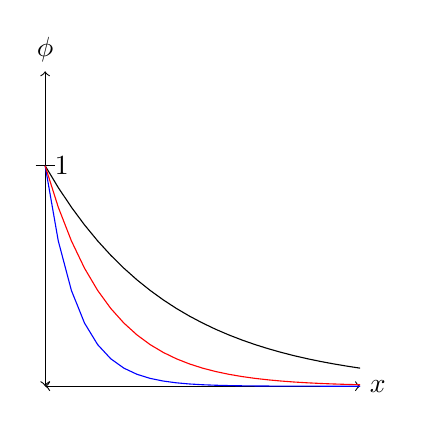
\begin{tikzpicture}[scale=0.4]
        \draw[<->] (0,0) -- (10,0);
        \node[right] at (10,0) {$x$};
        \draw[<->] (0,0) -- (0,10);
        \node[above] at (0,10) {$\phi$};
        \node[right] at (0,7) {$1$};
        \draw (-0.3,7) -- (0.3,7);
        \draw[blue, domain=0:10] plot(\x, {7*exp(-\x)});
        \draw[black, domain=0:10] plot(\x, {7*exp(-\x/4)});
        \draw[red, domain=0:10] plot(\x, {7*exp(-\x/2)});
    \end{tikzpicture}
    \caption{This is a snapshot, note time progression goes blue $\to$ red $\to$ black.}
    \label{5.5.plot}
\end{figure}

Note that as $t \to \infty$ that the argument of the error function approaches $0$ and $\erfc(0) = 1$, so that means that as $t \to \infty$ everybody feels $\phi = 1$. 

This solution assumes instantaneous propagation, because at $t = \epsilon > 0$ the temperature at any $x < \infty$ is nonzero! This is obviously nonphysical. This tells us that our heat equation is nonphysical for small $t$ or large $x$. 

Let's return to the finite domain, with BCs and ICs $\phi(x,0) = 1, \phi(0,t) = 0 = \phi(L,t)$. By Laplace transform we already know the homogeneous solution looks like
\begin{equation}
    \Phi_{hom}(x,s) = Ae^{\sqrt{s}x/a} + Be^{-\sqrt{s}x/a}
\end{equation}
and our particular integral looks like
\begin{equation}
    \Phi_{part}(x,s) = \frac{1}{s}
\end{equation}
for our fully general solution $\Phi(x,s) = \Phi_{hom}(x,s) + \Phi_{part}(x,s)$. We can go through some algebra to find $A,B$ in terms of the BCs and ICs, but this expression ends up looking something like $\frac{\text{ugly}}{1 + e^{\text{something}}}$ which is really ugly to take the Laplace transform! (He really dosen't say much more about these expressions than ugly and something). We should expand the denominator as a Taylor series and inverse transform each term individually to obtain $\phi(x,s)$, which looks like
\begin{equation}
    \phi(x,t) = 1 - \erfc \frac{L-x}{2a\sqrt{t}} - \erfc\frac{x}{2a\sqrt{t}}+ \erfc \frac{2L-x}{2a\sqrt{t}} + \erfc\frac{L + x}{2a\sqrt{t}}- \erfc \frac{3L-x}{2a\sqrt{t}} - \erfc\frac{2L + x}{2a\sqrt{t}}+\dots
\end{equation}

We recognize this solution form to look like a set of infinite image rods! This is kind of cool, because we take a lot of infinite rods and cancel their contributions to produce the solution for a finite rod (we discuss this two paragraphs down). 

Recall though that both our separation of variables solution and our current solution in terms of $\erfc$ functions are summations. Which one is better then? Well, for small $t$ it is clear that the $\erfc$ converges much faster, because the solution as sum of cosines will converge slowly as $e^{-t^2} \approx 1$ when $t$ is small (examine the actual expression \eqref{5.5.sepvar}).

At the other end of the spectrum, if $t$ is large the Fourier expansion converges very quickly while $\erfc$ tends to $1$ so we prefer the Fourier expansion for large $t$!

More precisely, this method of images looks something like this. We start with the solution over $[0,\infty]$, but this doesn't satisfy $BCs$ at $x=1$ over our finite domain. We then add a source at $x=1$ to make the BCs work, but then we still don't satisfy BCs, so we can keep adding terms to come closer and closer to satisfying BCs (yeah, I don't quite understand this either). 

\chapter{5/7/14 --- Greens Functions, Fourier transform}

Let's now do what we did last class more generally. Consider initial conditions $\phi(x,0) = 0, \phi(0,t) = f(t)$ over $0 < x < \infty$. Recall that before we said $f(t) = 1$. If we again take the Laplace transform then we have ODE
\begin{equation}
    s\Phi(x,s) = a^2 \ptd{}{x}\Phi(x,s)\label{5.7.heat}
\end{equation}
over $0 < x < \infty$ but now the BC looks like
\begin{equation}
    \Phi(0,s) = F(s)
\end{equation}
for $F(s)$ the Laplace transform of $f(t)$. Recall then that the general solution looks like
\begin{align}
    \Phi_{hom}(x,s) = Ae^{\sqrt{s}x/a} + Be^{-\sqrt{s}x/a}
\end{align}

Recall that since we are solving over semi-infinite domain we know that $A = 0$ because we want nonexploding solution (BOOM!). Given then the boundary condition we see that
\begin{align}
    \Phi(x,s) &= F(s)e^{-\sqrt{s}x/a}
\end{align}

We then need to take the inverse Laplace transform. To do this we use convolution theorem for Laplace transforms
\begin{align}
    H(s) &= F(s)G(s)\\
    F(s) &= \int\limits_{0}^{t}f(t)e^{-st}\;dt\\
    G(s) &= \int\limits_{0}^{t}g(t)e^{-st}\;dt\\
    h(t) &= \int\limits_{0}^{t}f(t - \tau) g(\tau)\;d\tau\label{5.7.conv}
\end{align}

We know that $F(s) \to f(t)$ and by our little table last lecture $e^{-\sqrt{s}x/a} \to \frac{x}{2a\sqrt{\pi} \tau^{3/2}}e^{-x^2/4a^2\tau}$, so
\begin{align}
    \phi(x,t) &= \int\limits_{0}^{t}f(t - \tau)\frac{x}{2a\sqrt{\pi} \tau^{3/2}}e^{-x^2/4a^2\tau}\;d\tau\\
    &= \int\limits_{0}^{t}f(\tau)\frac{x}{2a\sqrt{\pi} (t-\tau)^{3/2}}e^{-x^2/4a^2(t-\tau)}\;d\tau\label{5.7.sol}
\end{align}

We can then identify the uglybutt expression above. We recall that any function $f(t) = \int\limits_{0}^{t}f(\tau)\delta(t-\tau)\;d\tau$ with $\delta$ the delta function, vanishing everywhere $t \neq \tau$ and integral $1$. We will be careful and define $\int\limits_{0}^{\infty}\delta(\tau)\;d\tau = 1$ so that it does what we want it to do even over the nonnegative domain (i.e. integrate to $1$). This carefulness is necessary because the $\delta$ function is typically defined only over $(-\infty,\infty)$.

We then look at what happens if $f(\tau)$ is a delta function, then it is clear that our ugly expression above is the Greens function! That is
\begin{equation}
    G(x,t-\tau) = \frac{x}{2a\sqrt{\pi} (t-\tau)^{3/2}}e^{-x^2/4a^2(t-\tau)}
\end{equation}

So we can then interpret $f(t)$ as a sum of delta functions, so then our above \eqref{5.7.sol} is then just intuitively the sum of the reaction of $\phi$ to a bunch of delta impulses with amplitude given by $f(\tau)$ summed over all $\tau$. In this way we can view the solution as a superposition of the reaction to these delta impulses!

We have examined the Laplace transform in the time domain, but we can also look at the Fourier transform in space domain! Suppose we again want to solve for the diffusion equation
\begin{equation}
    \pd{\phi}{t} = a^2 \ptd{\phi}{x}\label{5.7.diffuse}
\end{equation}
over $-\infty < x < \infty$. We then need an initial condition $\phi(x,0) = f(x)$, and the implicit BC for infinite domain is that $\phi(x,t)$ doesn't explode as $x \to \pm \infty$. We already know that we can solve it using Laplace transforms over all time, but we note that we can also solve using Fourier transform. We recall this to be
\begin{align}
    F(\lambda) &= \frac{1}{\sqrt{2\pi}}\int\limits_{-\infty}^{\infty}f(x)e^{-i\lambda x}\;dx\\
    f(x)  &= \frac{1}{\sqrt{2\pi}}\int\limits_{-\infty}^{\infty}F(\lambda)e^{i\lambda x}\;d\lambda\\
\end{align}

Let's first examine the effect of the Fourier transform on a derivative. We write
\begin{align}
    G(\lambda) &= \frac{1}{\sqrt{2\pi}}\int\limits_{-\infty}^{\infty}f'(x)e^{-i\lambda x}\;dx\\
    \text{{\tiny Integration by parts}} &= \frac{i\lambda}{\sqrt{2\pi}}\int\limits_{-\infty}^{\infty}f(x)e^{-i\lambda x}\;dx\\
    &= i\lambda F(\lambda)
\end{align}

Then the double derivative obviously transforms as $-\lambda^2 F(\lambda)$. 

Note that the integration by parts assumes that $f(x)$ and derivatives vanish as $x \to \pm \infty$. This isn't always true; we've only restricted to finite but not vanishing! This is solved by using a ``mollified'' function $f(x) e^{-\epsilon \abs{x}}$. We can use this function to ensure that the boundary term in the integration by parts (the term that doesn't involve the integral and is only evaluated at the endpoints) vanishes, and so our proof holds (we can obviously take $\epsilon \to 0$ after we're done with the integration by parts). Thus we won't have to worry too much; we'll just remember how the Fourier transform handles derivatives.

Let's take the initial condition $\phi(x,0) = \sin(\omega x), \omega > 0$. Then we multiply both sides of the heat equation by $\frac{1}{\sqrt{2\pi}}e^{-i\lambda x}$ and integrate both sides $dx$, effectively taking the Fourier transform. This gives us
\begin{align}
    \Phi(\lambda,t) &= A(\lambda)e^{-a^2\lambda^2t}\\
\end{align}
with $A(\lambda)$ defined by the initial condition's transform as
\begin{align}
    \Phi(\lambda,0) &= \frac{1}{\sqrt{2\pi}}\int\limits_{-\infty}^{\infty}e^{-i\lambda x}\sin \omega x\;dx
\end{align}

Hm. Since $\sin \omega x$ doesn't vanish, we must mollify the function. We thus transform instead $e^{-\epsilon \abs{x}}\sin \omega x$ and take the limit $\epsilon \to 0$, which gives us
\begin{align}
    \Phi(\lambda,0) &= \lim_{\epsilon \to 0}\frac{1}{i\sqrt{2\pi}} \left[ \frac{\epsilon}{(\lambda - \omega)^2 + \epsilon^2} - \frac{\epsilon}{(\lambda + \omega)^2 + \epsilon^2} \right]
\end{align}

This is still a tricky limit to take! We note that $\lambda \pm  \omega \neq 0$ produces vanishing limit, but $\lambda = \pm \omega$ is singular. This is then obviously a delta function in both cases, so then our initial condition looks like 
\begin{equation}
        \Phi(\lambda,0) = \frac{1}{i\sqrt{2\pi}} \left[ \pi \delta(\lambda - \omega) - \pi \delta(\lambda + \omega) \right]
\end{equation}
(note normalization $\pi$ arises only when we integrate over $\epsilon$ to find the exact height of the delta function). This then gives us our final solution
\begin{equation}
    \phi(x,t) = e^{-a^2 \omega^2 t}\sin \omega x
\end{equation}

Surprise! The heat equation maintains the modes (oscillation frequencies) in the initial condition. We could have anticipated this result from our earlier work in separation of variables.

This is then very easy to generalize to arbitrary initial condition $\phi(x,0) = f(x)$. We just need to compute the Fourier transform of $f(x)$ to $F(\lambda)$ and so
\begin{equation}
    \Phi(\lambda,t) = F(\lambda) e^{-a^2 \lambda^2 t}
\end{equation}

He just writes this equation down, but it should be easy to see comparing to our earlier result. We then need to observe the convolution theorem for Fourier transform, which is just given
\begin{align}
    \Phi(\lambda,t) &= F(\lambda)G(\lambda)\\
    \phi(x,t) &= \frac{1}{\sqrt{2\pi}}\int\limits_{-\infty}^{\infty}f(\xi) g(x-\xi)\;d\xi
\end{align}

Then we have
\begin{align}
    g(x,t) &= \frac{1}{\sqrt{2\pi}}\int\limits_{-\infty}^{\infty}e^{i\lambda x}e^{-a^2 \lambda^2 t}\;d\lambda\\
    &= \frac{1}{\sqrt{2a^2t}}e^{-\frac{x^2}{4a^2t}}
\end{align}
by simply performing the Gaussian integral (complete the square in the exponent, change variables) Finally, we can substitute this into the convolution formula and obtain our full expression
\begin{equation}
    \phi(x,t) = \frac{1}{2\sqrt{\pi a^2 t}}\int\limits_{-\infty}^{\infty}f(\xi)\exp\left\{ -\frac{(x-\xi)^2}{4a^2t} \right\}\;d\xi\label{5.7.FourierSol}
\end{equation}

Again we see that this is a superposition of the response of the system to arbitrary delta functions whose amplitudes are given by $f(\xi)$. So we can identify the Greens function
\begin{equation}
    G(x|\xi;t) = \frac{1}{2\sqrt{\pi a^2 t}}e^{-\frac{(x-\xi)^2}{4a^2 t}}
\end{equation}

We can check that the integral $\int\limits_{-\infty}^{\infty}G(x|\xi;t)\;dx = 1$. We suspect then that this Green's function is the solution to the heat equation under initial condition $\phi(x,0) = \delta(x-\xi)$. We can check this by Fourier transform; note that the Fourier transform of the $\delta$ function is simply $\frac{1}{\sqrt{2\pi}}e^{-i\lambda \xi}$ and so if we solve through over the exact same procedure as we got above we will find that $\phi(x,t) = G(x|\xi,t)$.

This procedure confirms our suspicion earlier, that if we treat $f(\xi)$ as a superposition of delta functions over a range of parameters $\xi$ and we integrate over all these delta functions $d\xi$ then we will recover the general solution! (I hope this makes sense, it's not easy to explain without jargon). 

Suppose that we now want to solve the same heat equation \eqref{5.7.diffuse} under semi-infinite interval $0 < x < \infty$. Then we need BCs $\phi(0,t) = f(t), \phi(\infty,t) < \infty$, and IC $\phi(x,0) = f(x)$. For now we'll just do $\phi(t,0) = 0$. 

The correct way to solve this is then to extend the function $\phi$ about $x=0$ such that $\phi(x) = -\phi(-x)$, due to the boundary condition, and then we can just solve the full domain function using the sine transform (since we know the cosine terms will vanish since the extended function is odd).

If we had Neumann boundary conditions, so $\phi_x(0,t) = 0$, then it would be natural to solve with a cosine transform.

Let $f(x)$ exhibit sine transform $F_s(\lambda)$ and cosine transform $F_c(\lambda)$ then
\begin{align}
    F_s(\lambda) &= \sqrt{\frac{2}{\pi}}\int\limits_0^{\infty}f(x)\sin(x\lambda)\;dx\\
    F_c(\lambda) &= \sqrt{\frac{2}{\pi}}\int\limits_0^{\infty}f(x)\cos(x\lambda)\;dx\\
    % f'(x) \to -\lambda F_c(\lambda) & f''(x) \to \sqrt{\frac{2}{\pi}}\lambda f(0) - \lambda^2 F_s(\lambda)\label{5.7.sin}\\
    % f'(x) \to -\sqrt{\frac{2}{\pi}}f(0) + \lambda F_s(\lambda) & f''(x) \to -\sqrt{\frac{2}{\pi}}f'(0) - \lambda^2 F_c(\lambda)\label{5.7.cosin}
    \sqrt{\frac{2}{\pi}}\int\limits_{0}^{\infty}y''(x)\cos(kx)\;dx &= -k^2 Y_c(k) - \sqrt{\frac{2}{\pi}}y'(0)\label{5.7.cosin}\\
    \sqrt{\frac{2}{\pi}}\int\limits_{0}^{\infty}y''(x)\sin(kx)\;dx &= -k^2 Y_s(k) - \sqrt{\frac{2}{\pi}}ky(0)\label{5.7.sin}
\end{align}
where my sloppy notation is meant to denote that the  derivatives of the function have sine transform \eqref{5.7.sin} and cosine transform \eqref{5.7.cosin}. It is then clear why we use sine for Dirichlet boundary (given $f(0)$) and cosine for Neumann boundary (given $f'(0)$). It's not hard to show that the general solution under sine transform (we choose one) is given by
\begin{equation}
    \phi(x,t) = \frac{1}{4\pi at}\int\limits_{0}^{\infty}f(x')\left[ e^{-(x - x')^2/4at} - e^{-(x + x')^2/4at} \right]\;dx'
\end{equation}

Hey look, it looks very much so like our general solution from the full domain Fourier transform given by \eqref{5.7.FourierSol}.

\chapter{5/9/14 --- Separation of variables/eigenfunction expansion, Method of finite transforms}

Recall that last lecture we found solution to the heat equation $\pd{u}{t} = k\ptd{u}{x}$ over $0 < x < L$ to be
\begin{equation}
    u(x,t) = \sum_{n=1}^{\infty}c_ne^{-\frac{n^2\pi^2 kt}{L^2}}\sin \frac{n\pi x}{L}
\end{equation}

We use $c_n$ to satisfy initial conditions; note that the $\sin$ term already satisfies the boundary conditions. In order then to satisfy the inital conditions we find for initial condition $g(x)$
\begin{align}
    u(x,0) = g(x) &= \sum_{n=1}^{\infty} c_n \sin \frac{n\pi x}{L}\\
    c_n &= \frac{2}{L}\int\limits_{0}^{L}g(x)\sin \frac{n\pi x}{L}\;d
\end{align}

We ask how this converges? Parseval's theorem states that
\begin{equation}
    \int\limits_{0}^{L}\left[ g(x) - \sum_{n=0}^{N}c_n\sin \frac{n\pi x}{L} \right]^2\;dx = \sum_{N+1}^{\infty}c_n^2 \to 0
\end{equation}
as $N \to \infty$ as long as $g(x)$ is square integrable. Thus the series will converge in the mean square sense when $g(x)$ is square integrable.

In time though, the function decays faster than any power of $t$ for $t > 0$ because it is exponentially damped! This means that the series is always infinitely differentiable because it converges so damn quickly.

The idea of using a sum of separable functions leads us to examine general solutionss of form $u(x,t) = \alpha_n(t)\beta_n(x)$ (shout outs go to Albert for his fantastic notation). Note then that this produces in the heat equation
\begin{align}
    U_t &= \alpha'_n(t) \beta_n(x) & U_{xx} &= \alpha_n(t) \beta_{n}''(x)\\
    \alpha_n'(t)\beta_n(t) &= K\alpha_n(t)\beta_n''(x)\\
    \frac{\beta_n''(x)}{\beta_n(x)} &= \frac{\alpha_n'(t)}{k\alpha_n(t)} = -\lambda_n^2
\end{align}
where we choose the arbitrary constant that both separate terms must statisfy. We then know that the $\beta_n$ satisfy $S-L$ ODE $\beta_n''(x) + \lambda^2 \beta_n(x) = 0$ subject to $\beta_n(0) = \beta_n(L) = 0$. The solutions to this are clearly the sines, and this is how we can recover the separation of variables result by examining a sum of S-L eigenfunctions (I think he's trying hard to emphasize that this is different from straight up separation of variables, but I can't exactly see the big hoot; I guess this is an S-L eigenfunction expansion rather than just a separation of variables approach?).
\begin{figure}[!h]
    \centering
    \begin{tikzpicture}[scale=0.4]
        \draw (-0.5,-1) -- (-0.5,-2);
        \draw (0.5,-1) -- (0.5,-2);
        \draw(-1.5,-2.6) arc[radius = 3, start angle = 240, end angle = 300];
    \end{tikzpicture}
    \caption{Everything's better with a smiley, particularly one drawn as two lines and an arc!}
\end{figure}

If we have Neumann BCs (on $u_x(0,t), u_x(L,t)$) then we just have different S-L eigenfunctions, namely the cosines. Similarly, if we have mixed boundary conditions (mix of Dirichlet/Neumann) then we should use the appropriate combination of the sines/cosines to construct our eigenfunctions and expand. 

Now consider the heat equation with a source term $\phi_t = a^2 \phi_{xx} + w(x,t)$ over $0 < x < L$ such that $\phi(0,t) = \phi(L,t) = 0$ Dirichlet BCs. Obviously we cannot apply separation of variables directly into the PDE, but we can make an insightful guess and explore series solution
\begin{equation}
    \phi(x,t) = \sum_{n}^{}\alpha_n(t)\sin \frac{n\pi x}{L}
\end{equation}
or more precisely the series expansion for the homogeneous case. Then in the PDE we obtain
\begin{align}
    \sum_{n=0}^{\infty}\pd{\alpha_n}{t}\sin \frac{n\pi x}{L} &= a^2 \sum_{n=1}^{\infty} \alpha_n(t) \left( -\frac{n^2 \pi^2}{L^2} \right)\sin \frac{n\pi x}{L} + w(x,t)\label{5.9.PDE}
\end{align}

This doesn't look so easy, but the clear way to proceed from here is to expand $w(x,t)$ in terms of the sine eigenfunctions, the same eigenbasis (which we know is a complete basis). We thus assume $w$ of form
\begin{align}
    w(x,t) &= \sum_{n=1}^{\infty}w_n(t)\sin \frac{n\pi x}{L}\\
    w_n(t) &= \frac{2}{L}\int\limits_{0}^{t}w(x,t) \sin \frac{n\pi x}{l}\;dx
\end{align}
which plugging back into \eqref{5.9.PDE} we obtain
\begin{align}
    \sum_{n=0}^{\infty}\pd{\alpha_n}{t}\sin \frac{n\pi x}{L} &= \sum_{n=1}^{\infty}\alpha_n(t) \left( w_n(t) - a^2 \frac{n^2\pi^2}{L^2} \right)\sin \frac{n\pi x}{L}\\
    \pd{\alpha_n}{t} &= w_n(t) - a^2\frac{n^2 \pi^2}{L^2}
\end{align}

We can solve this directly via the methods in 95b to obtain
\begin{equation}
    \alpha_n(t) = C_n e^{-\frac{n^2 \pi^2 a^2 t}{L^2}} + e^{-\frac{n^2 \pi^2 a^2 t}{L^2}}\int\limits_{0}^{t}e^{\frac{n^2 \pi^2 a^2 \tau}{L^2}}W_n(\tau)\;d\tau
\end{equation}

The first term is the homogeneous solution of the ODE and the second term is the particular integral for the inhomogeneous case. We note exactly one degree of freedom for the first order ODE as we expect. We can also find $C_n$ in terms of the intial condition $\phi(x,0) = g(x)$ by hitting $g(x)$ with the appropriate Fourier decomposition (didn't copy it down exactly, but obviously some integral against sines).

We can in general handle the inhomogeneous PDE via an ansatz of the form $\phi = \phi_{s} + \phi_{p}$ with $\phi_s$ the homogeneous solution and $\phi_p$ the particular integral, and oftentimes we will want to decompose both $\phi_0, \phi_p$ with the same eigenfunction decomposition. Recall that this only helps because the PDE is linear!

Let's examine the convergence of our series solution. We note that the homogeneous term converges as well as it always did (exponentially decaying in $t$ so for positive $t$ we decay exponentially coefficients!), but the inhomogeneous? There's a growing exponential on the inside! Recall
\begin{align}
    \phi_p(x,t) &= \sum_{n=1}^{\infty}G_n\sin \frac{n\pi x}{L}\\
    G_n &= e^{-\frac{n^2 \pi^2 a^2 t}{L^2}}\int\limits_{0}^{t}e^{\frac{n^2 \pi^2 a^2 \tau}{L^2}}w_n(\tau)\;d\tau\label{5.9.inhom}
\end{align}

We are saved by the fact that the $w_n$ decay at slowest as $n^{-1}$, such as the example function
\begin{align}
    w(x,t) &= 1 & w_n &= \frac{2}{n\pi}\left[ 1 - \cos n\pi \right]
\end{align}

It turns out that if we use these $w_n$ and integrate \eqref{5.9.inhom} then we will find $G_n \sim n^{-3}$, with the extra factors of $n$ coming out of an integration by parts. Namely
\begin{align}
    G_n &= e^{-\frac{n^2 \pi^2 a^2 t}{L^2}}\int\limits_{0}^{t}e^{\frac{n^2 \pi^2 a^2 \tau}{L^2}}\frac{2}{n\pi}\left[ 1 - \cos n\pi \right]\;d\tau\\
    &= \frac{L^2}{n^2 \pi^2 a^2}e^{-\frac{n^2 \pi^2 a^2 t}{L^2}} \left[ e^{\frac{n^2 \pi^2 a^2 \tau}{L^2}} - 1 \right] \left[ \frac{2}{n\pi}\left( 1 - \cos n\pi \right) \right]\\
    &= \frac{2L^2}{n^3 \pi^3 a^2} \left[ 1 - e^{-\frac{n^2 \pi^2 a^2 \tau}{L^2}} \right] \left[ 1 - \cos n\pi \right]
\end{align}

So despite the Gibbs phenomenon inherent in sinusoidal expansion of $w(x,t)$ (basically, recall that since $w=1$ doesn't satisfy the same BCs as the sines the expansion converges super poorly), we can still obtain a series solution that converges fast enough to be a solution to the heat equation.

What about inhomogeneous BC? Consider if $\phi(0,t) = g(t), \phi(L,t) = h(t)$ subject to initial conditions $\phi(x,0) = f(x)$ for the full heat equation $\phi_t = a^2 \phi_{xx} + w(x,t)$. The correct way to handle these inhomogeneous BCs is to make a charge of variables to the solution
\begin{equation}
    \phi(x,t) = \psi(x,t) + g(t) I_0(x) + h(t)I_L(x)
\end{equation}
with $I_0(0) = 1, I_0(L) = 0, I_L(0) = 0, I_L(L) = 1$ but no other constraints on these functions. Then $\psi$ satisfies homogeneous BCs and we can unleash the full fury of all the techniques we've learned thusfar. A simple choice is $I_0(x) = 1 - x/L, I_L = x/L$. This is called the method of finite transforms (also covered in 95b).

GOLDEN QUOTE. Professor Hou: ``So Prof. Rizza told me that since we lost some ground we needed to cover all three techniques in three lectures. I told him I couldn't do it, but apparently I've managed to finish. I hope it's all been clear, sorry if the pace has been too fast, and good luck!'' Awww. 
\chapter{5/12/14-5/14/14 --- Heat equation in multiple dimension}

Today we will derive heat equation in multiple dimensions. I'm not going to copy down the derivation, we obtain the following equation
\begin{equation}
    \pd{u}{t} = k\nabla^2 u + Q
\end{equation}

Uniqueness holds when we have a Dirichlet BC, $u(x,y,z,t) = f(x,y,z,t)$ for $x,y,z \in \partial R$ or a Neumann BC $-K_0 \vec{\nabla} u \cdot \hat{n} = g(x,y,z,t)$ for $x,y,z \in \partial R$. We will often abbreviate $\vec{\nabla} u \cdot \hat{n} = \pd{u}{\hat{n}}$ the \emph{normal derivative}. 

The equilibrium case looks like $\nabla^ u = -\frac{Q}{k}$, the Poisson equation. Then if $Q = 0$ then we have the Laplace equation.

The heat equation should use whatever geometry makes most sense, so either cylindrical/spherical coordinates too. Careful though, the Laplacian is not well defined at $r=0$ in these coordinate systems! (inb4 delta functions).

Let's try to solve the heat equation in 2D through separation of variables $u(x,y,t) = X(x)Y(y)T(t)$. Substituting into the heat equation we again get
\begin{equation}
    \frac{T_t}{kT} = \frac{X_{xx}}{X} + \frac{Y_{yy}}{Y}
\end{equation}

We expect $\frac{T_t}{kT} = -\lambda$ so we have $T(t) = e^{-k\lambda t}$. Let's consider over Dirichlet BCs $X(0) = X(L) = Y(0) = Y(M) =0$. We can then get $X,Y$ to satisfy the boundary conditions by $X = \sin \frac{n\pi x}{L}, Y = \sin \frac{m \pi y}{M}$. Then the \emph{modes} that we have look like
\begin{align}
    \phi_{mn} &= \sin \frac{n\pi x}{L}\sin \frac{m\pi y}{M}\\
    U &= \sum\limits_{}^{}C_{mn}\phi_{mn}
\end{align}
with coefficients $C_{mn}$ determined by initial conditions $U(x,y,0)$ and taking appropriate integral (looks scary, just orthogonality).
\begin{equation}
    \int\limits_{0}^{L}dx\;\int\limits_{0}^{M}dy\;U(x,y,0) \sin \frac{n' \pi x}{L} \sin \frac{m' \pi y}{M} = \sum\limits_{n,m}^{}C_{nm}\int\limits_{0}^{L}dx\;\int\limits_{0}^{M}dy\; \sin \frac{n' \pi x}{L}\sin \frac{n\pi x}{L} \sin \frac{m' \pi y}{M}\sin \frac{m\pi y}{M}
\end{equation}

We can also use separation of variables to solve in polar coordinates (since we're still too stoopid to go to 3D), which if we use the correct Laplacian and make the same time ansatz as before we obtain
\begin{align}
    -\lambda^2 = \frac{1}{rR}\pd{}{r}\left( r \pd{R}{r} \right) + \frac{1}{r^2}\frac{\Theta_{\theta\theta}}{\Theta}
\end{align}

Then we can separate again and find $\Theta_{\theta\theta} = m^2\Theta$ assuming again constants whatnot stuff, and finally we obtain radial equation
\begin{align}
    \frac{1}{r}\rd{}{r}\left( r\rd{R}{r} \right) - \frac{m^2}{r^2}R + \lambda^2 R &= 0\\
    \rd{}{r}\left( r\rd{R}{r} \right) - \frac{m^2}{r}R + \lambda^2 rR &= 0
\end{align}
in Sturm-Liouville form. The solutions to these are the Bessel functions; we fix them by assuming $u(r_0) = 0$! The general solution can be found in the posted lecture notes, you get the idea.

For spherical coordinates we can still use separation of variables, go through Laplacian blah, we will ultimately discover that the $\theta, \phi$ parts go with the spherical harmonics while the $r$ part goes with the spherical Bessel function. Glhf, not taking notes on this stuff. Actually, the radial equation looks like
\begin{equation}
    \frac{1}{r^2}\rd{}{r}\left( r^2 \rd{R}{r} \right) - \frac{m}{r^2}R = \lambda R
\end{equation}
and we will treat instead of spherical harmonics the $\sin m\phi, \cos n\phi$ and $\Theta = P_{lm}$ the generalized Legendre polynomials.

\chapter{5/16/14 --- Helmholtz Equation}

Last class we solved the heat equation for vanishing Dirichlet boundary conditions with some arbitrary initial condition $f(x)$, and we discussed the square, circle, and sphere cases for various coordinate systems (teehee, didn't jot this down sorry). The overaching solution comprises three steps
\begin{itemize}
    \item Separate variables to change PDEs into ODE
    \item Use BCs to fix some set of S-L eigenfunctions by solving ODE
    \item Use S-L orthogonality to get coefficients of eigenfunctions from initial conditions
\end{itemize}

Today we will discuss the Helmholtz equation. It looks like the S-L operator but has eigenvalue degeneracy. 

Recall that our heat equation looked like $\partial_t U = \nabla^2 U$, which we solved via separation of variables ansatz $U = T(t) \phi(\vec{x})$. While before we separated $\phi$ as well, today we will examine directly what happens to $\phi$. The resulting equation that is satisfied when we plug $U$ into the heat equation looks like
\begin{equation}
    \nabla^2 \phi(\vec{r}) + \lambda \phi(\vec{r}) = 0
\end{equation}

This is the \emph{Helmholtz Equation}. Recall that in the wave equation it's just $\partial_{tt} U = \nabla^2 U$ and so if we plug in the same ansatz above we have te same Helmholtz equation in $\phi$ but just different time behavior (heat equation gives exponential solutions, wave equation gives oscillating). 

We will begin by solving the Helmholtz equation in a simple geometry, a 2D rectangle $L\times L$. Then the Helmholtz equation looks like
\begin{equation}
    \ptd{\phi}{x} + \ptd{\phi}{y} = -\lambda \phi
\end{equation}
and if we plug in $\phi(x,y) = X(x)Y(y)$ then we find that $\phi(x,y) = \sin \frac{n\pi x}{L}\sin \frac{m\pi y}{L}$ and so the eigenvalues look like $\lambda_{mn} = \frac{(n^2 + m^2) \pi^2}{L^2}$. Similar techniques can be found for other simple geometries we've already considered.

The Helmholtz operator is self-adjoint in the same way as the S-L operator. Recall the S-L operator looks like
\begin{align}
    \mathcal{L}u &= \left( p(x) u' \right)' + q(x)u
\end{align}
then the meaning of self-adjoint is that $\dotp{Lu}{v} = \dotp{u}{Lv}$ with this inner product defined $\int\limits_{0}^{1}(\mathcal{L}u) v\;dx$. We showed the self-adjoint-ness of the S-L operator last term; refer to 95b notes (specifically, from 2/14/14 lecture, the Lagrange identity). 

We can show that the Helmholtz is self-adjoint too. Recall that $\vec{\nabla} \cdot \left( a\vec{b} \right) = a\vec{\nabla} \cdot \vec{b} + (\vec{\nabla}a) \cdot \vec{b}$, so then we can find
\begin{align}
    \vec{\nabla} \cdot (u \vec{\nabla} v) &= u \nabla^2 v + \vec{\nabla} u \cdot \vec{\nabla}v\\
    \vec{\nabla} \cdot (v \vec{\nabla} u) &= v \nabla^2 u + \vec{\nabla} v \cdot \vec{\nabla}u\\
    u \nabla^2 v - v\nabla^2 u &= \vec{\nabla} \cdot \left( u \vec{\nabla} v - v \vec{\nabla}u \right)
\end{align}

Then integrating over $R$, we can turn the right hand side into a surface integral via divergence theorem
\begin{align}
    \int\limits_{R}^{}u \nabla^2 v - v\nabla^2 u d\vec{r}&= \int\limits_{\partial R}^{}\left( u \vec{\nabla} v - v \vec{\nabla}u \right) \cdot \hat{n} dS\\
    &= \int\limits_{\partial R}^{}\left( u \pd{v}{\hat{n}} - v\pd{u}{\hat{n}} \right)dS
\end{align}

Then if our BCs are such that the RHS vanishes (either Dirichlet or Neumann could work) then we obtain
\begin{equation}
    \int\limits_{R}^{}u \nabla^2 v - v\nabla^2 u\;d\vec{r} = 0
\end{equation}
which is sufficient to show self-adjointness of the Helmholtz equation (this may seem like the self-adjointness of the Laplacian, but recall that we required BCs, and the Helmholtz equation includes these BCs as well). Recall from linear algebra that self-adjoint operators then have real eigenvalues and orthogonal eigenvectors. 

However, there is a key difference between the Helmholtz and S-L operators. The S-L had nondegenerate eigenvalues, while the Helmholtz can degenerate eigenvalues (the root cause for this can be usually traced to the homogeneity of space and the symmetry of the Laplacian). This means that there is oftentimes a space of eigenfunctions that correspond to the same eigenvalues, so we need to orthogonalize this space to find a set of basis vectors (consider the linear algebra equivalent when a matrix with degenerate eigenvalues would have a space of eigenvectors that needed to be orthogonalized). The procedure to find this basis is the same as in linear algebra: Gram-Schmidt.

Consider $\phi_n$ a set of eigenfunctions with same eigenvalue under the Helmholtz operator. Then the crux of the argument is that we choose $\psi_1 = \phi_1$ and then $\psi_2 = \phi_2 - \frac{\dotp{\phi_1}{\phi_2}}{\dotp{\phi_1}{\phi_1}}\phi_1$ (we subtract out the parallel component so that they are orthogonal) and repeat for all $n$ eigenfunctions. Such procedures typically make one very very sad in algebra.

Let's see how the Rayleigh quotient comes about (she talk about how this is pretty useless, but it'll be useful for us on the exam lol). Let's multiply $\phi$ on both sides of the Helmholtz equation to obtain
\begin{align}
    \nabla^2 \phi + \lambda \phi &= 0\\
    \lambda \phi^2 &= -\phi \nabla^2 \phi\\
    \lambda = -\frac{\int\limits_{R}^{}\phi \nabla^2 \phi\;d\vec{r}}{\int\limits_{R}^{}\phi^2\;d\vec{r}}
\end{align}

The denominator looks quite pretty, but the numerator isn't very symmetric. Let's integrate by parts (never forget the great Dan Meiron ``the most powerful technique in applied mathematics'') and obtain
\begin{align}
    \lambda &= -\frac{\int\limits_{R}^{}\vec{\nabla} \cdot \left( \phi \vec{\nabla}\phi \right)d\vec{r} - \int\limits_{R}^{}\abs{\vec{\nabla} \phi}^2\;d\vec{r}}{\int\limits_{R}^{}\phi^2\;d\vec{r}}
\end{align}

Then of course if we use divergence theorem and if we have homogeneous Dirichlet/Neumann ($=0$) BCs then we have
\begin{align}
    \lambda = \frac{\int\limits_{R}^{}\abs{\vec{\nabla}\phi}^2\;d\vec{r}}{\int\limits_{R}^{}\phi^2\;d\vec{r}}
\end{align}

This is \emph{Rayleigh's quotient}. Thus we know that $\lambda$ must be positive, which we already knew because self-adjoint Helmholtz operator! Note we cannot have $\lambda = 0$ because this implies $\vec{\nabla} \phi = 0$ everywhere, which is a trivial solution for Dirichlet BCs ($\phi = 0$) and still a pretty boring flat solution for Neumann BCs ($\phi = C$).

The most important use of Rayleigh quotient is to estimate eigenvalues. Then if we find the minimum Raleigh quotient, this must be the eigenvalue of the lowest eigenvalue of the Helmholtz equation (I want to say ground state, physicist problems). The equality is not difficult to prove; if we plug $\phi_1$ into the Rayleigh quotient we find $\mathrm{min} \lambda \leq \lambda_1$ and if we write down any arbitrary superposition we find that $\lambda \geq \lambda_1$ which shows the equality.
\chapter{5/16/14 --- Midterm Review Session}

List of topics
\begin{itemize}
    \item Series solutions/separation of variables
        \begin{itemize}
            \item with nonhomogeneous BCs
            \item with source terms
            \item in extra dimensions
            \item using various other eigenexpansions such as Bessel functions
        \end{itemize}
    \item Transforms: fourier, laplace, sine, cosine
    \item Problems will be mostly about the heat equation
\end{itemize}

It is difficult to tell what method to use for what problems some times. Let's do some practice problems
\begin{itemize}
    \item $u_t = u_{xx}$ over $0 < x < \infty$ for $u(0,t) = g(t)$ and $u(x,0) = f(x)$: valid solutions include
        \begin{itemize}
            \item Laplace transform in time, solve ODE for $U(x,s)$ and inverse transform.
            \item Sine transform, because Dirichlet BC ($u(0,t) = g(t)$ as opposed to $u'(0,t)$).
            \item If we tried to Laplace transform in space, we recall that the Laplace transform acts on the second derivative $dx^2$ while producing both $u(x=0)$ and $u'(x=0)$ terms, which is problematic! Therefore, since we don't have conditions on $u'$ we cannot Laplace transform in space.
            \item If our problem were over $-\infty < x < \infty$ then obviously a full Fourier transform is more natural, because nothing else has BC dependences that work well with the $\infty$s.
        \end{itemize}
    \item What about $u_t = u_{xx} + u_{yy} + u_x + q(x,y,t)$ with $u(0,y,t) = u(1,y,t) = u(x,0,t) = u(x,1,t) = 0$ and $u(x,y,0) = f(x,y)$?
        \begin{itemize}
            \item A sine transform (or any transform for that matter) might not work well (as was suggested by a classmate) because it doesn't play well over the finite domain.
            \item A sine series expansion seems to get a little closer, but there will still be some random terms floating around that don't quite cancel well, it seems.
            \item A separation of variables approach seems best, so that we will obtain some S-L problem whose eigenfunctions are the natural expansion for the problem. 
        \end{itemize}
\end{itemize}

Let's go ahead and work out this second example first before we discuss anything further. We begin of course by ignoring the source term and solving for the general solution (so also ignore ICs). This means that we make ansatz $u = T(t)X(x)Y(y)$, which plugged through our PDE gives
\begin{align}
    T'XY &= TX''Y + TXY'' + TX'Y\\
    \frac{T'}{T} &= \frac{X''}{X} + \frac{Y''}{Y} + \frac{X'}{X}
\end{align}

We then generally want to separate this into a spatial coordinate on one side and everything else on the other. It is then natural that we should want to isolate $Y(y)$ first because it obeys a less complicated ODE, and we obtain
\begin{align}
    \frac{T'}{T} - \frac{X''}{X} - \frac{X'}{X} &= \frac{Y''}{Y} = \lambda
\end{align}
which obviously yields solutions $Y'' = \lambda Y$. We then know obviously that $\lambda$ will be negative, so we solve and obtain $Y_n(y) = \sin(n\pi y)$ with $\lambda = -n^2\pi^2$. Then we have
\begin{equation}
    \frac{T'}{T} - \frac{X''}{X} - \frac{X'}{X} = -n^2\pi^2
\end{equation}
and then we write again
\begin{equation}
    \frac{T'}{T} = \frac{X''}{X} = \frac{X'}{X}  -n^2\pi^2 = \mu
\end{equation}
with $\mu$ a new constant, and we solve for $X$ which obeys ODE
\begin{equation}
    X'' + X' - (n^2\pi^2 + \mu)X = 0\label{5.16.reviewODE}
\end{equation}
subject to $X(0) = X(1) = 0$. Let's take this to S-L form $\left(\rd{}{x}\left( p(x)\rd{y}{x} \right) - q(x)y + \lambda r(x)y = 0\right)$ so that we can understand the nature of the solutions (it doesn't help us solve for $\mu$ eigenvalues though), and we obtain form
\begin{equation}
    \rd{}{x}\left( e^xX' \right) - (n\pi)^2e^xX - \mu e^xX = 0
\end{equation}
with $\mu$ our eigenvalue. Note that $r(x) = e^x$ our integrating factor! This will be important in the orthogonality relations that we must use later. But to actually solve the ODE we return to form \eqref{5.16.reviewODE}, which is a second order ODE with constant coefficients, which solves out easily (via ansatz $X = e^{mx}$)to
\begin{align}
    0 &= m^2 + m - \left( (n\pi)^2 + \mu \right)\\
    m_\pm &= -\frac{1}{2} \pm \sqrt{\frac{1}{4} + (n\pi)^2 + \mu}\\
    X(x) &= c_1e^{m_x+} + c_2e^{m_-x}
\end{align}

We then apply BCs to this, $X(0) = X(1) = 0$. Then it is first evident that $m_{\pm} \in \mathbb{R}$ cannot satisfy this, so the square root must be imaginary. This means our full solution looks like sines and cosines
\begin{equation}
    X(x) = e^{-\frac{x}{2}}\left[ c_3\sin\left( x\frac{\sqrt{\frac{1}{4} + (n\pi)^2 + \mu}}{i} \right) + c_4\cos\left(x\frac{\sqrt{\frac{1}{4} + (n\pi)^2}+\mu}{i}\right) \right]
\end{equation}

Wow that's a mouthful! But secretly, the cosines fall out because $X(0) = 0$, and $X(1) = 0$ bounds the sine term and we find (obviously we should have chosen $\mu \to -\mu$)
\begin{align}
    m\pi &= \sqrt{-\frac{1}{4} - (n\pi)^2 - \mu}\\
    X_m(x) &= e^{-\frac{x}{2}}\sin mx
\end{align}

Then finally,we know that these $X_m$ are orthogonal such that $\int\limits_{0}^{1}X_mX_{m'}e^x\;dx = \delta_{mm'}\int\limits_{0}^{1}X_m^2e^x\;dx$. ${3 \over 2} \frac{3}{2}$.

Finally we can execute the series expansion. We write
\begin{align}
    u(x,y,t) &= \sum\limits_{n,m=1}^{\infty}a_{nm}(t)X_m(x)Y_n(y) & q(x,y,t) &=\sum\limits_{n,m=1}^{\infty}q_{nm}(t)X_m(x)Y_n(y) & f(x,y) &= \sum\limits_{n,m=1}^{\infty}f_{nm}X_m(x)Y_n(y)
\end{align}
with the coefficients $f_{mn}, q_{mn}$ determined by
\begin{align}
    f_{n,m} &= \frac{\int\limits_{0}^{1}\int\limits_{0}^{1}f(x,y)e^xX_m(x)Y_n(y)\;dx\;dy}{\int\limits_{0}^{1}\int\limits_{0}^{1}\sin^2(n\pi x)\sin^2(m\pi y)\;dx\;dy}
\end{align}
and similarly for $q$. Note the integrating factor goes away because of the $e^{-\frac{x}{2}}$ in the $X_m$. Our equation then looks like (entire equation is summed over $n,m$)
\begin{equation}
    a_{nm}'(t)X_m(x)Y_n(y) = a_nm(t)\left(X_m''(x) + X'(x)\right)Y_n(y) + a_nm(t)X_m(x)Y_n'(y) + q_nm(t)X_m(x)Y_n(y)
\end{equation}

But then recall that $X_m'' + X_m' = (n\pi)^2 + \mu)X_m = \left(-\frac{1}{4} - (m\pi)^2\right)X_m$ so (we can make a further simplification by $Y_n''(y) = -n^2\pi^2 Y_n(y)$) we get
\begin{align}
    a_{nm}'(t)X_m(x)Y_n(y) &= a_{nm}(t)\left(-\frac{1}{4} - (m\pi)^2\right)X_m(x)Y_n(y) - n^2\pi^2 a_{nm}(t)X_m(x)Y_n(y) + q_{nm}(t)X_m(x)Y_n(y)\\
    a_{nm}'(t) &= a_{nm}(t)\left(-\frac{1}{4} - (m\pi)^2\right) - n^2\pi^2 a_{nm}(t) + q_{nm}(t)\\
\end{align}

This gives us enough information to determine $a_{nm}(t)$ and thus determine $u(x,y,t)$.

Let's solve a new example now, using Fourier transforms. We will exhibit PDE $u_t = ku_{xx} + cu_x$ over $-\infty < x < \infty$ and $u(x,0) = f(x)$. We transform the PDE and obtain (denote $\mathcal{F}(u) = U$ the Fourier transform of $u$)
\begin{align}
    U_t = -\lambda^2 kU + ic\lambda U\label{5.16.ODE2}
\end{align}
recalling the Fourier transform acting on derivative $\mathcal{F}(u_x) = i\lambda \mathcal{F}(u)$. This is seen through the following derivation (integration by parts carry hard)
\begin{align}
    \mathcal{F}(f'(x)) &= \frac{1}{\sqrt{2\pi}}\int\limits_{-\infty}^{\infty}f'(x)e^{-i\lambda x}\;dx\\
    &= \frac{1}{\sqrt{2\pi}}\left[ f(x)e^{-i\lambda x}\Bigg|_{-\infty}^\infty - (-i\lambda)\int\limits_{-\infty}^{\infty}f(x)e^{-i\lambda x}\;dx \right]\\
    &= \frac{1}{\sqrt{2\pi}}\int\limits_{-\infty}^{\infty}i\lambda f(x)e^{-i\lambda x}\;dx
\end{align}
where the boundary term vanishes because implicit BCs $f(\pm \infty)$ doesn't explode. 

Let's go back now to the ODE after having taken the Fourier transform, \eqref{5.16.ODE2}. This is an ezpz ODE, with solution
\begin{equation}
    U(t,\lambda) = A(\lambda)e^{(-\lambda^2k + ic\lambda)t}
\end{equation}

We then must constrain $A(\lambda)$, via our ICs! We take the Fourier transform of the IC $u(x,0) = f(x) \Rightarrow U(x,\lambda = 0) = F(\lambda)$. Then clearly
\begin{equation}
    U(t,\lambda) = F(\lambda)e^{(-\lambda^2k + ic\lambda)t}
\end{equation}

We must then take the inverse Fourier transform. It is then natural that we convolve for $u(t,x)$, and since we know that Gaussians Fourier transform to Gaussians (specifically, we will use $\mathcal{F}(e^{-ax^2}) = \sqrt{\pi/a}e^{-\lambda^2/4m}$ though maybe this is wrong(I think it's wrong by a factor of $1/\sqrt{2\pi}$ but w/e)) we are almost there. But first, we prove cursorily that $\mathcal{F}(f(\alpha - \beta)) = e^{-i\lambda \beta}\mathcal{F}(f(\alpha))$. 

We are finally ready then to convolve. Let $g(x,t)$ be the inverse Fourier transform of $e^{-\lambda^2 kt}$ (which she tried to write down earlier but I think is incorrect), then (note $*$ denotes convolution)
\begin{align}
    u = f(x + ct)*g(x,t) = \frac{1}{\sqrt{2\pi}}\int\limits_{-\infty}^{\infty}f(w + ct) g(x-w,t)\;dw
\end{align}

Good luck!
\chapter{5/21/14 --- Wave Equation!}

The wave equation in 1D looks like $\ptd{u}{t} = c(x)^2 \ptd{u}{x}$, with $c(x)$ a positive function of $x$ that describes propagation speed.

We can derive the wave equation carefully by considering the usual tightly stretched string that is displaced slightly from equilibrium, and we can eventually find
\begin{equation}
    F \approx \abs{T}\ptd{u}{x}\Delta x \hat{j}
\end{equation}

Then by Newton's second law $F = m\ddot{x} = \rho \Delta x \ptd{u}{t}$ we finaly obtain
\begin{equation}
    \ptd{u}{x} = \frac{\rho}{\abs{T}}\ptd{u}{t}
\end{equation}

Yeah, nobody really cares about the derivation unless you're a physicist, but the wave equation itself is super important! Note that this implies waves travel with speed $\sqrt{\frac{\rho}{T}}$. 

Let's look into the wave equation $\ptd{u}{t} = c^2 \ptd{u}{x}$ over $-\infty < x < \infty$ for $t > 0$ subject to ICs $u(x,0) = h(x), \pd{u}{t}(x,0) = p(x)$ (note that we now need two ICs)! We will solve this by first changing variable $\xi = x + ct, \eta = x - ct$ and seek a solution $\phi(\xi, \eta) = u\left(\frac{\xi + \eta}{2}, \frac{\xi - \eta}{2}\right)$. Substituting into our PDE turns out to yield
\begin{equation}
    \frac{\partial^2 \phi}{\partial \xi \partial \eta} = 0
\end{equation}

This then tells us that $\phi$ must be a sum of two functions $\alpha(\xi),\beta(\eta)$, giving that $u(x,t) = \alpha(x + ct) + \beta(x - ct)$. We then apply our ICs to determine our $\alpha, \beta$ and we find
\begin{align}
    u(x,0) &= \alpha(x) + \beta(x) = h(x)\\
    \pd{u}{t}(x,0) &= c\pd{\alpha}{\xi} - c\pd{\beta}{\eta} = c\pd{\alpha}{x} - c\pd{\beta}{x}= p(x)
\end{align}

Differentiating the first one and solving we find
\begin{align}
    \pd{\alpha}{x} &= \frac{p(x)}{2c} + \frac{h'(x)}{2} & \pd{\beta}{x} &= -\frac{p(x)}{2c} + \frac{h'(x)}{2}\\
    \alpha &= \int\limits_{}^{x}\frac{p(x')}{2c}\;dx' + \frac{h(x)}{2} + C & \beta &= -\int\limits_{}^{x}\frac{p(x')}{2c}\;dx' + \frac{h(x)}{2} - C
\end{align}

This gives our fully general form for $u(x,t)$
\begin{equation}
    u(x,t) = \frac{1}{2}\left[ h(x  + ct) + h(x - ct) \right] + \frac{1}{2c}\left[ \int\limits_{x-ct}^{x+ct}p(x')\;dx' \right]
\end{equation}
which is called the \emph{D'Alembert's solution} to the 1D wave equation. 

We can examine some special cases
\begin{itemize}
    \item $u(x,0) = h(x), \rd{u}{t}(x,0) = 0$, then we have $u(x,t) = \frac{h(x + ct) + h(x-ct)}{2}$. Note that the ICs propagate outwards no more quickly than $c$, introducing the idea of a \emph{region of influence}. 
    \item $h = 0,$, then $u(x,t) = \frac{1}{2c}\int\limits_{x-ct}^{x+ct}p(x')\;dx'$, this is the idea of \emph{domain dependence}, which states that the value of $u$ depends on previous values of $u$ within some domain around it (I think this is basically the same as region of influence).  
\end{itemize}

Let's now examine the wave equation in a finite domain, still 1D, still subject to $u(t=0) = h(x), u'(t=0) = p(x)$. We will give it now some BCs, there being the usual two cases Dirichlet and Neumann, at the endpoints $[0,L]$. 
\chapter{5/23/14 --- Solving 1D wave equation}

Note that the final will probably have longer time limit but will still be about same difficulty; just to make sure we have enough time to finish! How kind of him.

Solving 1D bounded wave equation. Let's examine $\ptd{u}{t} = c^2 \ptd{u}{x}$ over $0 \leq x \leq L$ and $t > 0$ with $c$ some positive constant. We will use BCs $u(0,t) = u(L,t) = 0$ and ICs $u(x,0) = h(x), \pd{u}{t}(x,0) = p(x)$ over $0 < x < L$.

We will solve using separation of variables, the ansatz $u(x,t) = \sum\limits_{n=1}^{\infty}\alpha_n(t) \beta_n(x)$ where we will guess $\beta_n(x)$ to be $\sin \frac{n\pi x}{L}$ for $n \in \mathbb{N}$. 

Then to solve for $\alpha_n(t)$ we use the method of \emph{finite transforms} (wait, I could have sworn this was to eliminate inhomogeneous BCs, but now it's just referring to transforms by orthogonal functions over a finite domain. This nomenclature makes more sense, but am I missing something?). We multiply both sides by $\sin \frac{n\pi x}{L}$ and integrate to obtain
\begin{align}
    \int\limits_{0}^{L}\rtd{u}{t}\sin \frac{n\pi x}{L}\;dx &= c^2 \int\limits_{0}^{L}\ptd{u}{x}\sin \frac{n\pi x}{L}\;dx\\
    \int\limits_{0}^{L}\left(\sum\limits_{n=1}^{\infty}\alpha_n(t)\sin \frac{n\pi x}{L}\right)\sin \frac{n\pi x}{L}\;dx&= -\frac{c^2 n^2 \pi^2}{L^2}\int\limits_{0}^{L}\left(\sum\limits_{n=1}^{\infty}\alpha_n(t)\sin \frac{n\pi x}{L}\right)\sin \frac{n\pi x}{L}\;dx\\
    \ddot{\alpha}_n = -\frac{c^2 n^2 \pi^2}{L^2}\alpha_n(t)
\end{align}
abusing orthogonality. Applying then our ICs we find that 
\begin{align}
    u(x,0) &= \sum\limits_{n=1}^{\infty} \alpha_n(0) \sin \frac{n\pi x}{L} = h(x) & \rd{u}{t}(x,0) &= \sum\limits_{n=1}^{\infty}\pd{\alpha_n(0)}{t}\sin \frac{n\pi x}{L} = p(x)
\end{align}

We can then decompose $h(x), p(x)$ into its Fourier components $p(x) = \sum\limits_{n=1}^{\infty}p_n\sin \frac{n\pi x}{L}, h(x) = h_n \sin\frac{n\pi x}{L}$ and obtain solution for our coefficients
\begin{align}
    \alpha_n(t) = h_n\cos \frac{n\pi ct}{L} + p_n\left( \frac{L}{n\pi c} \right)\sin \frac{n\pi ct}{L}
\end{align}
and substitute back and obtain
\begin{equation}
    u(x,t) = \sum\limits_{n=1}^{\infty}\left[ h_n\cos \frac{n\pi ct}{L} + p_n\left( \frac{L}{n\pi c} \right)\sin \frac{n\pi ct}{L} \right]\sin \frac{n\pi x}{L}
\end{equation}

Let's then examine the form of our solution, a superposition of the terms $\sin \frac{n\pi ct}{L}\sin \frac{n\pi x}{L}$ and $\cos \frac{n\pi ct}{L}\sin \frac{n\pi x}{L}$. We call these then the \emph{normal modes} of the solution with \emph{characteristic frequency} $\frac{\pi c}{L}$. 

Now let's examine the wave equation with forcing, which looks like $\ptd{u}{t} = c^2 \ptd{u}{x} + f(x,t)$. Let's use the same BCs, ICs as before and the same ansatz. Let's decompose the driving force $f(x,t) = \sum\limits_{n=1}^{\infty}f_n(t)\sin \frac{n\pi x}{L}$ and thus we arrive at the ODE for coefficents $\alpha$
\begin{equation}
    \rtd{\alpha_n}{t} = \frac{n^2 \pi^2 c^2}{L^2}\alpha_n + f_n(t)
\end{equation}

This then leads to full solution
\begin{equation}
    u(x,t) = \sum\limits_{n=1}^{\infty}\left[ h_n\cos \frac{n\pi ct}{L} + p_n\left( \frac{L}{n\pi c} \right)\sin \frac{n\pi ct}{L} + \frac{L}{n\pi c}\int\limits_{0}^{t}\sin \frac{n\pi c(t-\tau)}{L}f_n(\tau)\;d\tau\right]\sin \frac{n\pi x}{L}
\end{equation}
where we just solve the ODE above (he omits the solution because it's ODE territory not PDE territory). 

Let's then examine what happens on resonance (beat Pokemon again woohoo!). If our external force takes on form $f(x,t) = \sin \frac{N\pi ct}{L}\sin \frac{N\pi x}{L}$ where we force at one of the normal modes, then the coefficients take on form
\begin{align}
    \alpha_N(t) &= \frac{L}{N\pi c}\int\limits_{0}^{t}\sin \frac{N\pi c(t\tau)}{L}\sin \frac{N\pi c\tau}{L}\;d\tau\\
    &= \frac{L}{2NLc}\sin \frac{N\pi ct}{L}\int\limits_{0}^{t}\sin \frac{2Nc\tau}{L}\;d\tau - \frac{L}{N\pi c}\cos \frac{N \pi ct}{L}\int\limits_{0}^{t}\sin^2\left( \frac{N \pi c\tau}{L} \right)\;d\tau\\
    \int\limits_{0}^{t}\sin^2 \frac{N\pi c\tau}{L}\;d\tau &= \int\limits_{0}^{t}\frac{1}{2}\left( 1 - \cos \frac{2N\pi c\tau}{L} \right)\;d\tau\\
    &= \frac{t}{2} - \frac{L}{2N\pi c}\sin \frac{2N\pi ct}{L}
\end{align}
We note then that the coefficient $\alpha_N$ will increase linearly with time! (This are called \emph{secular growth} in physics) This then means that our $u(x,t)$ has a term that grows linearly with time as well, such that it looks like
\begin{equation}
    u(x,t) = Q(x,t) - \frac{t}{2}\left( \frac{L}{N\pi c} \right)\cos \frac{N\pi ct}{L}\sin \frac{N\pi x}{L}
\end{equation}
with $Q(x,t)$ being the other terms in $u(x,t)$.

Note that secular behavior is only possible in the wave equation; in the heat equation, as long as the heat source is not infinite we will never have exploding growth, but small forcing to wave equation can result in huge amplitudes, i.e. Tacoma Narrows bridge kaboom.

We've thusfar only talked about homogeneous Dirichlet BCs. We can talk a bit about how to solve other BCs, but we won't actually work through them. Suppose we have forced wave equation subject to the following cases
\begin{itemize}
    \item Homogeneous Neumann BCs --- $\pd{u}{x}(0,t) = \pd{u}{x}(L,t) = 0$, then the preferred approach is to expand in the ansatz $u(x,t) = \sum\limits_{n=0}^{\infty} \alpha_n(t)\cos \frac{n\pi x}{L}$; note the sum starts from $0$ instead, and we use cosines.
    \item Fully inhomogeneous BCs --- $u(0,t) = g(t), u(L,t) = h(t)$, then we use \emph{method of finite transforms} (why is this called the same thing as above??) to turn this into homogeneous BCs. 
\end{itemize}

All y'all jerks who ain't comin' to class, y'all suck.
\chapter{5/28/14 --- Green's function solution to Poisson Equation}

Recall that the Green's function $G$ for a linear operator $L$ is such that $LG(x,x_0) = \delta(x-x_0)$. Recall that the delta function has its usual sifting property.

We can then look at the Green's Function for the Poisson equation $\nabla^2 u = f(\vec{x})$. A useful identity for the Poisson Equation is is Green's third identity
\begin{equation}
    \iiint\limits_D u\nabla^2v - v\nabla^2u\; dV = \iint\limits_{\partial D} \left(u\vec{\nabla}v - v\vec{\nabla}u\right) \cdot \hat{n}\;dS
\end{equation}

Now we are looking for a solution to $\nabla^2 G(\vec{x},\vec{x}_0) = \delta(\vec{x} - \vec{x}_0$ subject to $G(\vec{x}, \vec{x}_0) = 0$. Then if we throw Green's third identity at this we obtain
\begin{align}
    \iiint\limits_D u\nabla^2G - G\nabla^2u\; dV &= \iint\limits_{\partial D} \left(u\vec{\nabla}G - G\vec{\nabla}u\right)\cdot \hat{n}\; dS\label{5.28.Greens}
\end{align}

Then by our BCs we find the right hand side vanishes so we obtain
\begin{align}
    \iiint\limits_D \left[ u \delta(\vec{x} - \vec{x}_0) - Gf(\vec{x}) \right]d^3\vec{x} &= 0\\
    \iiint\limits_D G(\vec{x}, \vec{x}_0) f(\vec{x}) d^3\vec{x} &= u(\vec{x}_0)
\end{align}

This then shows that we can obtain our general solution (apparently flipping $\vec{x} \leftrightarrow \vec{x}_0$ isn't always allowed, so there's a proof in the lecutre notes)
\begin{equation}
    u(\vec{x}) = \iiint\limits_D G(\vec{x}, \vec{x}_0) f(\vec{x}_0) d^3\vec{x}_0
\end{equation}

Roughly, the reason that we can flip this is because $G(\vec{x}, \vec{x}_0)$ is symmetric about its arguments. 

Now, let's examine the inhomogeneous BCs case, where $u(\vec{x}) = h(\vec{x})$ on the boundary. Then we go back to \eqref{5.28.Greens} and instead obtain
\begin{align}
    \iiint\limits_D \left[ u(\vec{x}) \delta(\vec{x} - \vec{x}_0) - G(\vec{x}, \vec{x}_0) f(\vec{x}) \right]d\vec{x} &= \iint\limits_{\partial D}h(\vec{x}) \vec{\nabla}G \cdot \hat{n}d\vec{x}\\
    \iiint\limits_D G(\vec{x}, \vec{x}_0) f(\vec{x})d\vec{x} + \iint\limits_{\partial D}h(\vec{x}) \vec{\nabla}G \cdot \hat{n} d\vec{x} &= u(\vec{x}_0)
\end{align}
and again flipping the variables because stuff is symmetric we get our general solution
\begin{equation}
    u(\vec{x}) = \iiint\limits_D G(\vec{x}, \vec{x}_0) f(\vec{x}_0)d\vec{x}_0 + \iint\limits_{\partial D}h(\vec{x}_0) \vec{\nabla}G \cdot \hat{n} d\vec{x}_0
\end{equation}

Let's now do some simple cases. Examine first free space, which means we want to solve $\nabla^2 G = \delta(\vec{x} - \vec{x}_0)$. Since the problem is isotropic fully, we can choose any arbitrary basis, and so we'll choose cylindrical coordinates since we'll work in 2D. This then gives us our Poisson equation
\begin{align}
    \frac{1}{r}\pd{}{r} \left( r \pd{G}{r} \right) + \frac{1}{r^2}\ptd{G}{\theta} &= \frac{\delta(r)}{r}\\
    \frac{1}{r}\pd{}{r} \left( r \pd{G}{r} \right)  &= \frac{\delta(r)}{r}
\end{align}
since we know that $G$ must be rotationally symmetric. Solving the ODE then gives $G = c_1 + c_2 \ln r$.

We must then find $c_1, c_2$. Recall that $\iint \nabla^2 G d\vec{x}= 1$, and we can use divergence theorem to get to
\begin{align}
    \iint \nabla^2 G d\vec{x} &= \int \pd{G}{n}dS = 1\\
    &= \int\limits_{0}^{2\pi}\pd{G}{r}r\;d\theta
\end{align}
which gives that $c_2 = \frac{1}{2\pi}$. We can then choose $c_1 = 0$, so our full Green's function just looks like $G = \frac{\ln r}{2\pi}$. 

\chapter{5/30/14 --- Final information, Greens functions again}

Last day! Undergrad final will be posted on Wednesday 6/11 at 1400 and due on Friday 6/13 at 1600. Final will account for $40\%$ of total grade, only take home portion, cumulative with focus on content from end of term. Exam will have somewhere around 4-6 problems and will be about 5-6 hours (shouldn't take so long). There will be a final review session, TBD. Don't forget TQFRs so we can all thank Jerry and the other TAs for their hard work since Adam's passing. 

From last time we solved for the Greens function for Poisson Equation $\nabla^2 u = f(\vec{x})$ in 2D, which is just solving $\nabla^2 G(\vec{x}, \vec{x}_0) = \delta(\vec{x} - \vec{x}_0)$. Then we eventually arrived at
\begin{align}
    G(\vec{x}, \vec{x}_0) = \frac{1}{2\pi}\ln \abs{\vec{x} - \vec{x}_0}
\end{align}

Howe then do we get a solution for $u(\vec{x})$? We use Green's third formula
\begin{align}
    \int\limits_D \left[ u \nabla^2G - G\nabla^2u \right]d\tau &= \int\limits_{\partial D} \left[ u\vec{\nabla} G - G\vec{\nabla}u \right]\cdot \hat{n}d\tau'
\end{align}

Then over our infinite domain the boundary integral vanishes and we obtain
\begin{align}
    u(\vec{x}) &= \frac{1}{2\pi}\iint f(\vec{x}_0) \ln \abs{\vec{x} - \vec{x}_0}d\vec{x}_0
\end{align}
in two-dimensions. Note that this holds only if $\lim_{r \to \infty}r\left( u \rd{G}{r} - G\rd{u}{r} \right) = 0$, which is the condition for which the boundary integral can vanish. 

What's kinda handy about Greens functions it's an integral so we can do it numerically. This is the end of the course material that we're expected to know.

Let's do a quick course recap to see what we've covered in this class
\begin{itemize}
    \item Tensor analysis, including
        \begin{itemize}
            \item Vectors in a basis
            \item Change of basis
            \item Introduced tensors as linear mappings of vectors, or as linear operators
        \end{itemize}
    \item Intro to PDEs
        \begin{itemize}
            \item Many cannot be analytically solved
            \item Investigated heat/wave equations
            \item Separation of variables
            \item Similarity solution
            \item Series expansion
            \item Laplace/Fourier/sine/cosine transform
            \item Greens functions
        \end{itemize}
    \item Multidimensional PDEs
        \begin{itemize}
            \item Laplace Equation
            \item Poisson Equation
            \item Helmholz Equation
        \end{itemize}
\end{itemize}

``Moving forward,'' things that we could have investigated are nonsimple domains for the heat/wave equations (anything but box, sphere, pole, etc.) and numerical methods. 

\chapter{6/03/14 --- Final review!}

Anything from this term can be on the final exam, including
\begin{itemize}
    \item Index Notation
    \item Curvilinear coordinates
    \item Series solutions to Laplace/Wave/Heat equation
    \item Fourier/Laplace transforms
    \item d'Alembert's solution
    \item Helholtz equation
    \item Greens Functions
\end{itemize}

Notation notes: $\hat{e}_1, \hat{e}_2, \hat{e}_3$ and $\hat{x}, \hat{y}, \hat{z}$ will be used interchangably.

\section{Index notation}
First, we'll speed through index notation from the beginning of term. Vectors go $v_i\hat{e}_i$. For example, exhibit a function $f(x_1, x_2, x_3) = x_ix_i$, then 
\begin{align}
    \left[ \vec{\nabla}f \right]_i &= \pd{}{x_j}\left( x_i x_i \right)\\
    &= x_i\pd{x_i}{x_j} + \pd{x_i}{x_j}x_i\\
    &= 2x_j
\end{align}
noting that $\pd{x_i}{x_j} = \delta_{ij}$ Kronecker delta.

\section{Curvilinear Coordinates}
Curvilinear coordinates are coordinates such as spherical or polar coordinates. In spherical coordinates we have $x = r\sin\theta\cos\phi, y = r\sin\theta\sin\phi, z = r\cos\theta$, and vectors go $\hat{r} \times \hat{\phi} = \hat{\theta}$ in terms of handedness.

We can also express our $\vec{\nabla}$ in our curvilinear coordinates, e.g. $\vec{\nabla}f = \pd{f}{r}\hat{r} + \frac{1}{r}\pd{f}{\theta}\hat{\theta} + \frac{1}{r\sin\theta}\pd{f}{\phi}\hat{\phi}$. For example, using our same example from before $f(\vec{x}) = x_ix_i = r^2$, then we find that $\vec{\nabla}f = 2r\hat{r}$. But then we run into the ever-so-existential question \emph{what is $\hat{r}$}? We define it via the usual rule for change of basis (and normalization) to arrive at
\begin{align}
    \hat{r} &= \frac{\pd{}{r}\left( x_i\hat{e}_i \right)}{\abs{\pd{}{r}\left( x_i\hat{e}_i \right)}} \\
    &= \sin\theta\cos\phi \hat{e}_1 + \sin\theta\sin\phi\hat{e}_2 + \cos\theta \hat{e}_3\\
    2r\hat{r} &= 2x\hat{e}_1 + 2y\hat{e}_2 + 2z\hat{e}_3 = 2x_i\hat{e}_i
\end{align}

\section{Example problem: Green's function, Fourier transform}

Let's solve Laplace's equation in the half-plane, so $\nabla^2 u = 0$ for $y > 0, -\infty < x < \infty$ subject to BC $u(x,0) = f(x)$ and implicit BC $u \to 0$ as $\abs{x}, \abs{y} \to \infty$ (constraint that solutions make physical sense).

Let's start by solving using a Green's function. The free-space Green's function in 2D is given by (recall lecture notes)
\begin{align}
    G(\vec{x}, \vec{x}_0) = \frac{1}{2\pi}\ln \abs{\vec{x} - \vec{x}_0}
\end{align}

We then want to fudge this Green's function into a Green's function over just the half-plane (for Dirichlet BCs), and the correct way to do this is via the method of images. We arrive at
\begin{align}
    G(\vec{x}, \vec{x}_0) = \frac{1}{2\pi}\ln \abs{\frac{\vec{x} - \vec{x}_0}{\vec{x} - \vec{x}^*_0}}
\end{align}
where $\vec{x}_0^* = (x_0, -y_0)$. We can intuitively see this as placing an image source at $\vec{x}_0^*$ and combining its influence with $\vec{x}_0$ source, because the BC produces this ``image'' that is reflected across the boundary. We can use this sort of approach for any linear boundary.

We then use the Green's function using Green's third theorem which produces
\begin{align}
    u(\vec{x}) &= \iint\limits_D G\nabla^2u\; d\vec{x}_0 + \int\limits_{\partial D}^{}\left( u\vec{\nabla}G - G\vec{\nabla}u \right)\cdot \hat{n}\;dS\\
    &= \int\limits_{\partial D}^{}u\vec{\nabla}G \cdot \hat{n}\;dS
\end{align}
where we drop first term because $\nabla^2u = 0$ because Laplace's equation, and the second falls out because $G(\vec{x}, \vec{x}_0) = 0$ on the boundary (on the boundary, $x_0 = 0$ because we are evaluating when $\vec{x}_0 \in \partial D$ so $G$ vanishes). Then $\hat{n} = -\hat{y}$ we note, and so we obtain
\begin{align}
    u(\vec{x}) &= \int\limits_{-\infty}^{\infty}-u(x_0,0)\pd{G}{y_0}\;dx_0\\
    G &= \frac{1}{2\pi}\ln\abs{\frac{(x-x_0)^2 + (y-y_0)^2}{(x-x_0)^2 + (y + y_0)^2}}^{1/2}\\
    &= \frac{1}{4\pi}\ln\abs{\frac{(x-x_0)^2 + (y-y_0)^2}{(x-x_0)^2 + (y + y_0)^2}}\\
    \pd{G}{y_0} &= \frac{1}{4\pi}\frac{(x-x_0)^2 + (y + y_0)^2}{(x-x_0)^2 + (y-y_0)^2} \cdot \frac{-2\left( y-y_0 \right)\left[ (x-x_0)^2 + (y+y_0)^2 \right] - 2(y+y_0)\left[ (x-x_0)^2 + (y-y_0)^2 \right]}{\left((x-x_0)^2 + (y + y_0)^2\right)^2}\\
    &= -\frac{1}{2\pi}\left[ \frac{y-y_0}{(x-x_0)^2 + (y-y_0)^2} + \frac{y+y_0}{(x-x_0)^2 + (y+y_0)^2} \right]\\
    u(\vec{x}) &= -\int\limits_{-\infty}^{\infty}f(x_0)\pd{G}{y_0}\Bigg|_{y_0 = 0}\;dx_0\\
    &= \frac{1}{\pi}\int\limits_{-\infty}^{\infty}f(x_0)\left[ \frac{y}{\left( x-x_0 \right)^2 + y^2} \right]\;dx_0\label{Greensol}
\end{align}

Let's try this again using a Fourier transform. We obviously have to take the full Fourier transform (as opposed to sine/cosine) because we are looking at the domain $-\infty < x < \infty$. Let's define $\hat{u}$ the Fourier transform of $u$ then we obtain
\begin{align}
    u_{xx} + u_{yy} &= 0 &\Rightarrow&& -\lambda^2 \hat{u} + \hat{u}_{yy} &= 0\\
    u(x,0) &= f(x) &\Rightarrow&& \hat{u}(\lambda,0) &= \hat{f}(\lambda)
\end{align}

We thus have to solve $\hat{u}_{yy} = \lambda^2 \hat{u}$ which gives general solution $\hat{u} = A(\lambda)e^{\lambda y} + B(\lambda) e^{-\lambda y}$. Then if we want to satisfy the implicit BC $\hat{u}(y \to \infty) \to 0$ then we find the only solution must have form $\hat{u} = C(\lambda)e^{-\abs{\lambda}y}$ (She really waved her hands hard here; you should think of it as having the freedom to choose $A(\lambda), B(\lambda)$ such that BCs are satisfied, so we can choose them to be like step functions, so we can get rid of the exploding solutions at either $\lambda = \pm \infty$ by using the step function correctly. In other words, $e^{-\abs{\lambda} y}$ is still a linear combination of the homogeneous solutions and so still satisfies the ODE). Then we impose our last BC $\hat{u}(\lambda,0) = c(\lambda) = \hat{f}(\lambda)$ and we find our solution for the transformed space to be
\begin{align}
    \hat{u} &= \hat{f}(\lambda)e^{-\abs{\lambda}y}
\end{align}

Then we must invert the Fourier transform. In practice this is easiest to do via convolution; recall the convolution theorem looks like $u = \frac{1}{\sqrt{2\pi}}\int\limits_{-\infty}^{\infty}f(x_0)g(x-x_0,y)\;dx_0$ with $g$ the inverse Fourier transform of $e^{-\abs{\lambda}y}$.

We will check this against our previous answer by checking whether the Fourier transform of $e^{-\abs{\lambda }y}$ is actually $\sim \frac{y}{x^2 + y^2}$ as we found before in \eqref{Greensol} (we can set $x_0 = 0$). It's clear that we want to transform the latter function, because it's nice and analytic everywhere, rather than the former function. So we seek to find
\begin{align}
    \mathcal{F}\left( g(x,y) \right) = \frac{1}{\sqrt{2\pi}}\int\limits_{-\infty}^{\infty}\frac{y}{x^2 + y^2}e^{-i\lambda x}\;dx
\end{align}

We first examine for $\lambda > 0$, in which case we close the contour over the bottom half plane (in case it's not clear, this is easiest to evaluate using residues) which introduces a negative sign because the contour is \emph{clockwise}, and if $\lambda < 0$ we close in the top half plane. The choice of closure is done by seeing which way gets the contribution along the outside contribution to vanish. As an example, if $\lambda > 0$ then
\begin{align}
    \mathcal{F}\left( g(x,y) \right) &= 2\pi i\Res\left[ \dots \right](-1)\\
    &= 2\pi i \frac{1}{\sqrt{2\pi}}\frac{2y}{2iy} \sim e^{-\lambda y}
\end{align}
and so we see that (sorry, I'm too lazy to figure out the factors of $2\pi$) this will work out correctly (use $p/q'$ rule to evaluate residue). If $\lambda < 0$ we can repeat the same procedure and we find $\sim e^{\lambda y}$ and so we find the full transform goes like $\sim e^{-\abs{\lambda}y}$ up to some factors that Gemma worked out correctly in class, and so the two solutions agree.

\section{Example problem: Wave equation wih damping and source term on finite interval}

Let's exhibit our wave equation $u_{tt} + \nu u_t = c^2u_{xx} + q(x,t)$ over $0<x<1$ with ICs $u(x,0) = f(x), u_t(x,0) = g(x)$ and BCs $u(0) = u(1) = 0$.

We cannot do a Fourier transform because our domain in $x$ is finite; we could do a Laplace transform in time, but a series expansion seems the most intuitive way to solve this problem. We note because of BCs that sine expansion probably makes the most sense (satisfies the BCs), so let's write down the usual
\begin{align}
    u(x,t) &= \sum\limits_{n=1}^{\infty}a_n(t)\sin n\pi x&
    q(x,t) &= \sum\limits_{n=1}^{\infty}q_n(t) \sin n\pi x&
    f(x) &= \sum\limits_{n=1}^{\infty} f_n \sin n\pi x&
    g(x) &= \sum\limits_{n=1}^{\infty}g_n \sin n\pi x
\end{align}
and substituting it into the PDE gives (let's just write one summation symbol and spare the typist)
\begin{align}
    \sum\limits_{n=1}^{\infty}\Bigg\{ a_n''(t) \sin n\pi x + \nu a_n'(t)\sin n\pi x = -c^2n^2\pi^2a_n(t)\sin n\pi x + q_n(t)\sin n\pi x \Bigg\}
\end{align}

We can then read off an ODE for the $a_n$ as below
\begin{align}
    a_n''(t) + \nu a_n'(t) + c^2n^2\pi^2a_n(t) &= q_n(t)\label{ezODE}
\end{align}

This is a second-order ODE with constant coefficients, so we will first solve the homogeneous case and then find a particular solution. The homogeneous case is solved with ansatz $a(t) = e^{mt}$ which produces $m = -\frac{\nu}{2}\pm \sqrt{\left( \frac{\nu}{2} \right)^2 - c^2n^2\pi^2}$ when plugged through \eqref{ezODE}. Let's assume the non-oscillatory case, so small $\nu$ (specifically, such that $m$ is complex). Then we obtain
\begin{align}
    a_n^{(1)}(t) &= e^{-\frac{\nu}{2}t}\cos \omega_\lambda t & a_n^{(2)}(t) &= e^{-\frac{\nu}{2}t}\sin \omega_\lambda t
\end{align}
with $\omega_\lambda = \sqrt{c^2n^2\pi^2 - \left( \frac{\nu}{2} \right)^2}$.

These are our two homogeneous solutions, we will use variation of parameters to compute the the inhomogeneous solutions. The general formula is, recall,
\begin{align}
    y_p(t) &= -y_1(t)\int\limits_{0}^{t}\frac{y_2(t')q_n(t')}{W(y_1, y_2)}\;dt' + y_2(t)\int\limits_{0}^{t}\frac{y_1(t')q_n(t')}{W(y_1,y_2)}\;dt'\\
    W(y_1,y_2) &= \begin{vmatrix} a_n^{(1)} & a_n^{(2)}\\ \rd{}{t}a_n^{(1)} & \rd{}{t}a_n^{(2)}\end{vmatrix} = \dots = \omega_\lambda e^{-\nu t}\\
    a_n(t) &= -e^{-\frac{\nu}{2}t}\cos \omega_\lambda t \int\limits_{0}^{t}\frac{e^{\nu t_0}}{\omega_\lambda}q_n(t_0)e^{-\frac{\nu}{2}t_0}\sin \omega_\lambda t_0\;dt_0 + e^{-\frac{\nu}{2}t}\sin \omega_\lambda t \int\limits_{0}^{t}\frac{e^{\nu t_0}}{\omega_\lambda}q_n(t_0)e^{-\frac{\nu}{2}t_0}\cos \omega_\lambda t_0\;dt_0
\end{align}

Exercise to reader: solve out $a_n^{(p)}(t)$, and then subject the full general solution to BCs and we'll find something that looks like $a_n(t) =a_n^{(p)}(t) + f_n a_n^{(1)} + \xi(g_n)a_n^{(2)}$ with $\xi$ some big weird function.

\end{document}
